% !TEX root = main_org.tex
\chapter{Results}

\section{$SC(m,n)$ Results}


\subsection{$SC(3,2)$ and $SC(4,2)$}

The centrality dependence of $SC(4,2)$ and $SC(3,2)$ are presented in Fig.\ref{figs:sc}. Positive values of $SC(4,2)$ are observed for all measured centralities. This suggests a positive correlation between the event-by-event fluctuations of $v_2$ and $v_4$. It also indicates that finding $v_2$ larger than average($\langle v_2 \rangle$) in an event enhances the probability of finding $v_4$ larger than average($\langle v_4 \rangle$) in that event. On the other hand, the negative results of $SC(3,2)$ over all measured centralities show the anti-correlation between $v_2$ and $v_3$ flow harmonic magnitudes, which further implies that finding $v_2$ larger than average($v_2 > \langle v_2 \rangle$) enhancing the probability of finding smaller $v_3$ than average($v_3 < \langle v_3 \rangle$).


	
 	\begin{figure}[!p]
		\begin{center}
        	\resizebox{0.85\columnwidth}{!}{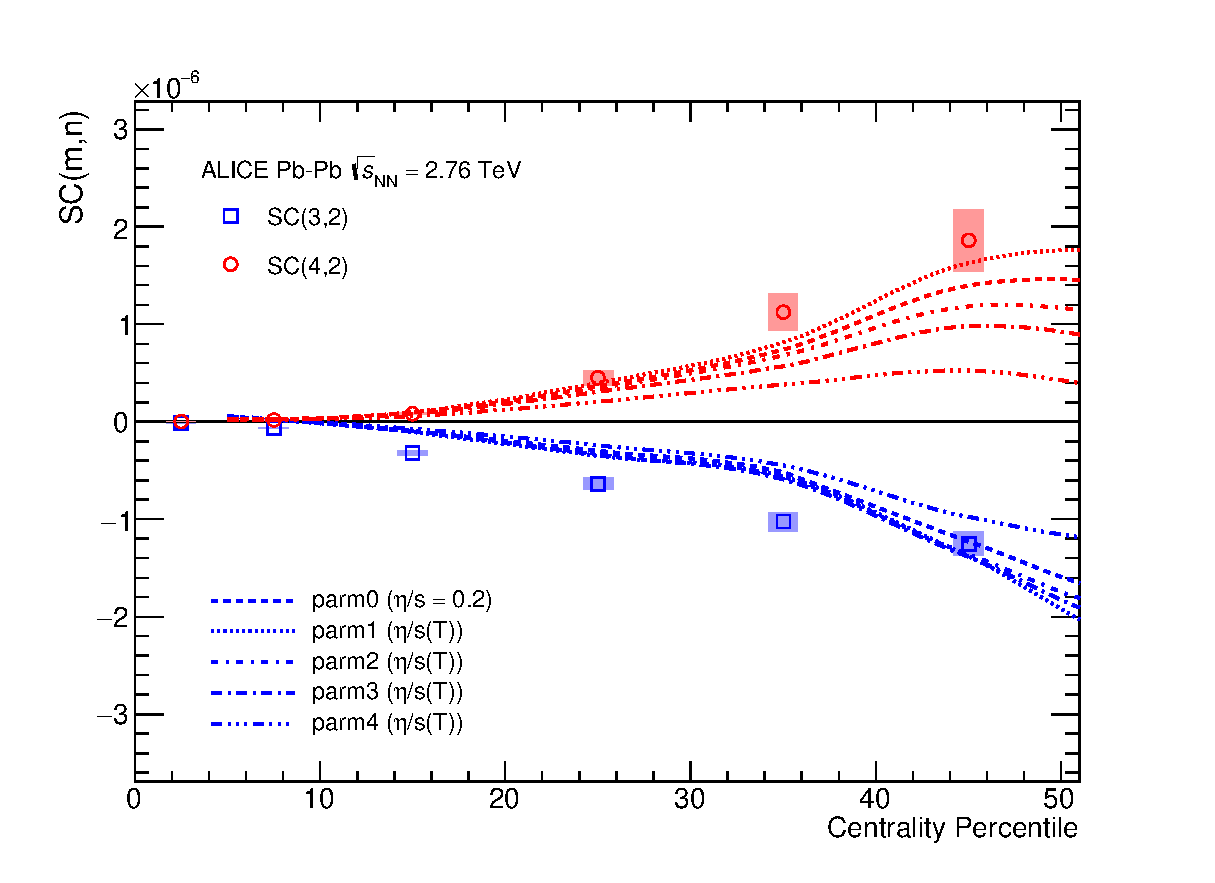
\includegraphics{figures/figs_results/fig1_QConly}}
        	\resizebox{0.85\columnwidth}{!}{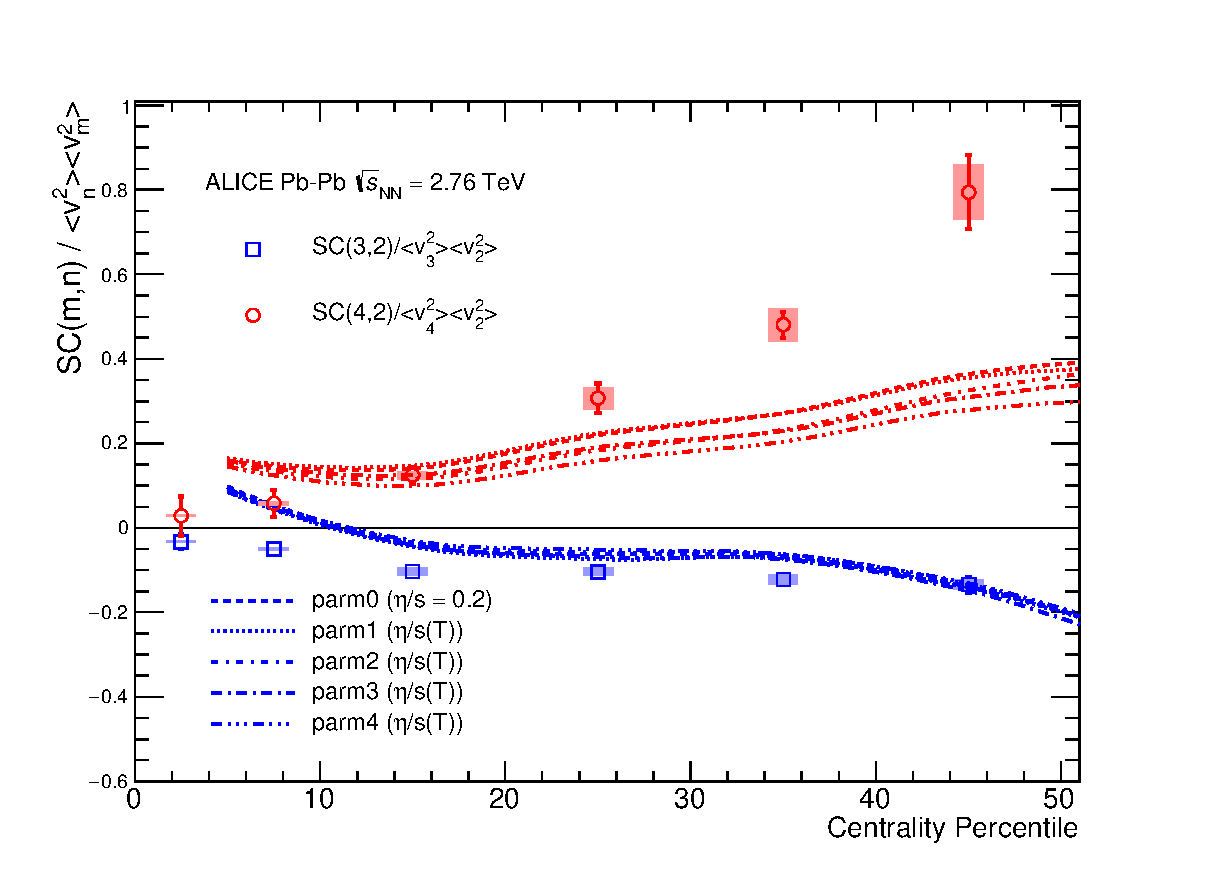
\includegraphics{figures/figs_results/fig1_QConly_norm}}
        \caption{The results of $SC(3,2)$(blue) and $SC(4,2)$(red) with ALICE Pb+Pb $\sqrt{S_{NN}}=2.76$TeV as function of collision centrality (Top). The $NSC(m,n)$ results which scaled with $\langle v_m^2 \rangle \langle v_n^2 \rangle $ were placed in Bottom. The dashed lines are hydrodynamic prediction from H. Niemi with various $\eta / s$ parametrizations \cite{Niemi:2015qia}  }
        \label{figs:sc}
        \end{center}   
     \end{figure}

As discussed and evaluated order-by-order in \cite{Gyulassy:1994ew}, general cumulant formalism is applicable to any correlators eliminating non-flow correlations up to order $2k$ by means of a cumulant expansion. Also when compared with HIJING simulation data\cite{PhysRevD.44.3501} does not include anisotropic collectivity, but has azimuthal correlations due to jet production (non-flow effects)\cite{Borghini:2000sa}.  It is found that both $$\langle \langle \cos{(m\varphi_1 + n\varphi_2 - m\varphi_3 - n\varphi_4)} \rangle \rangle = \langle v_m^2 v_n^2 \rangle $$ and  $$\langle \langle  \cos[m(\varphi_1 - \varphi_2)] \rangle \rangle \langle \langle  \cos[n(\varphi_1 - \varphi_2)] \rangle \rangle = \langle v_m^2 \rangle \langle v_n^2 \rangle$$ are not zero. However, the calculation of $SC(m,n)$ from HJING are compatible with zero for all centralities (even for higher $p_T$ as shown in Fig.\ref{fig:results_HIJING}) and it suggest that the $SC(m,n)$ are not coming from non-flow effects and insensitive to non-flow correlations.

Moreover, systematics study using the same charge combination pair technique has been done, which is another approach to estimate the non-flow effect. By using like-sign track selection method, we can eliminate ``flow cluster" effects due to charge conservation. As the result of systematic study, it was found that the difference between like-sign and all charged measurements are only few\% level and also we can found same trends (positive and negative correlation for $SC(4,2)$ and $SC(3,2)$) in like-sign results. This further illustrates that non-zero values of $SC(m,n)$ cannot be explained by non-flow effect, but confirms the existence of correlation (and anti-correlations) between $v_n$ and $v_m$ harmonics.

The $SC(m,n)$ results show that the correlation strength in both $SC(m,n)$ and $NSC(m,n)$ increase non-linearly up to centrality 50\%. 

	\begin{figure}[h]
		\begin{center}
        	\resizebox{0.45\columnwidth}{!}{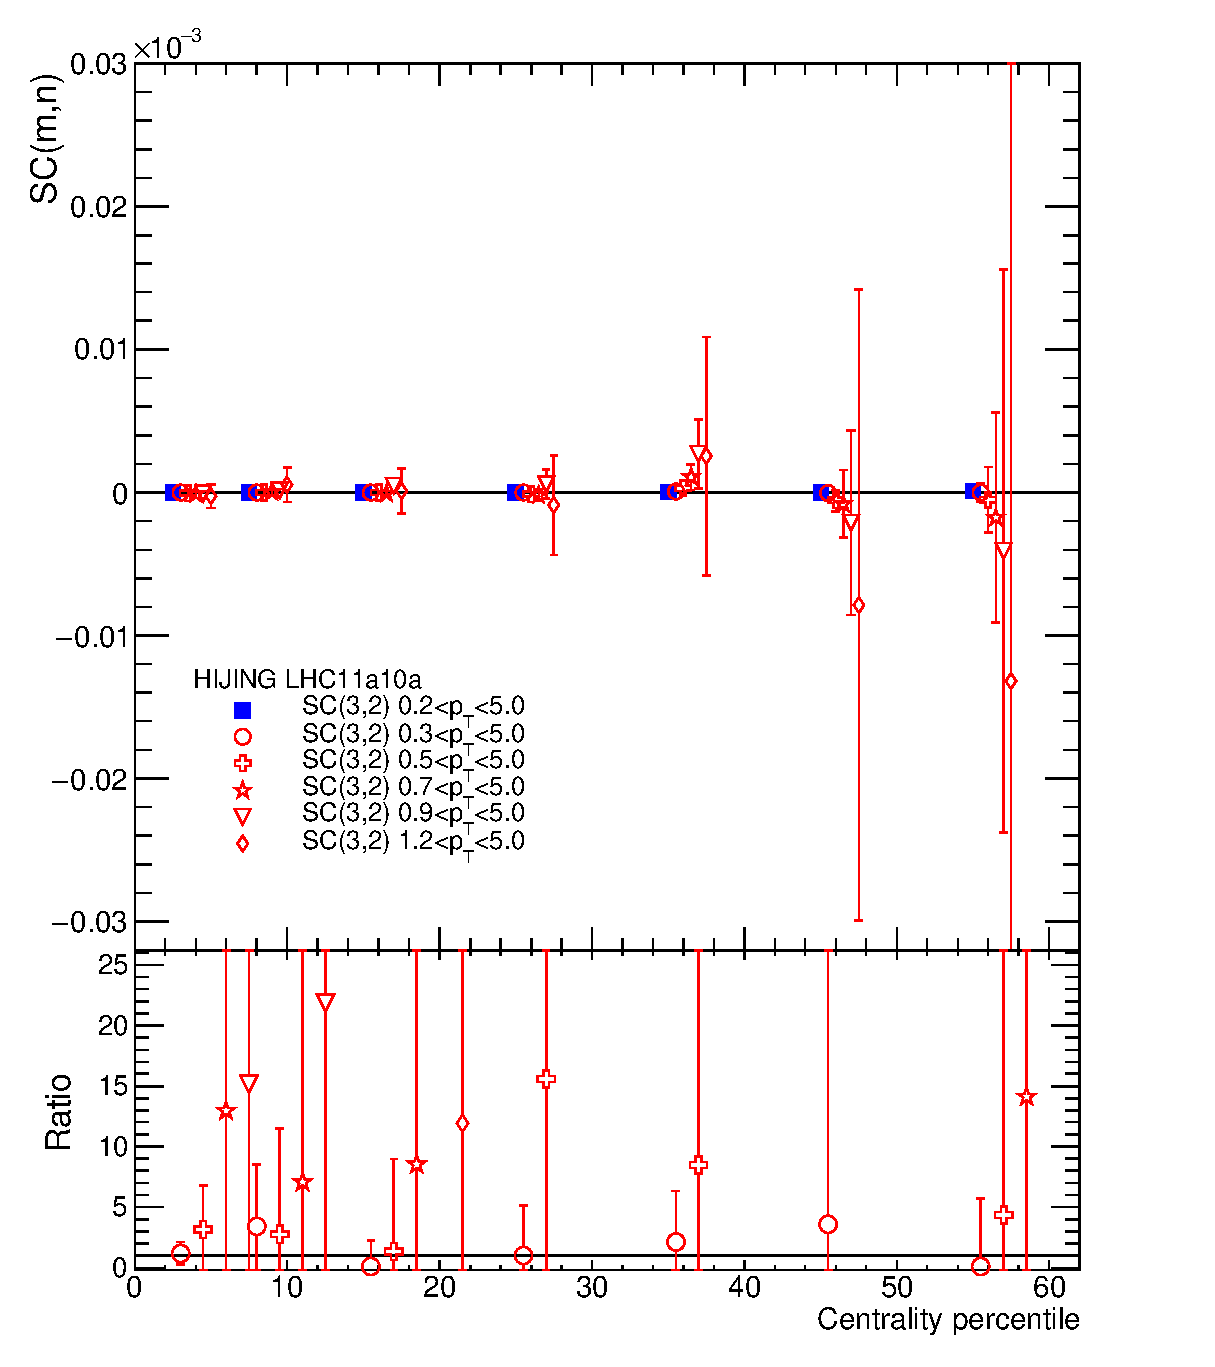
\includegraphics{figures/figs_results/SC_Comparison_SC32_HIJING_ptdep}}
        	\resizebox{0.45\columnwidth}{!}{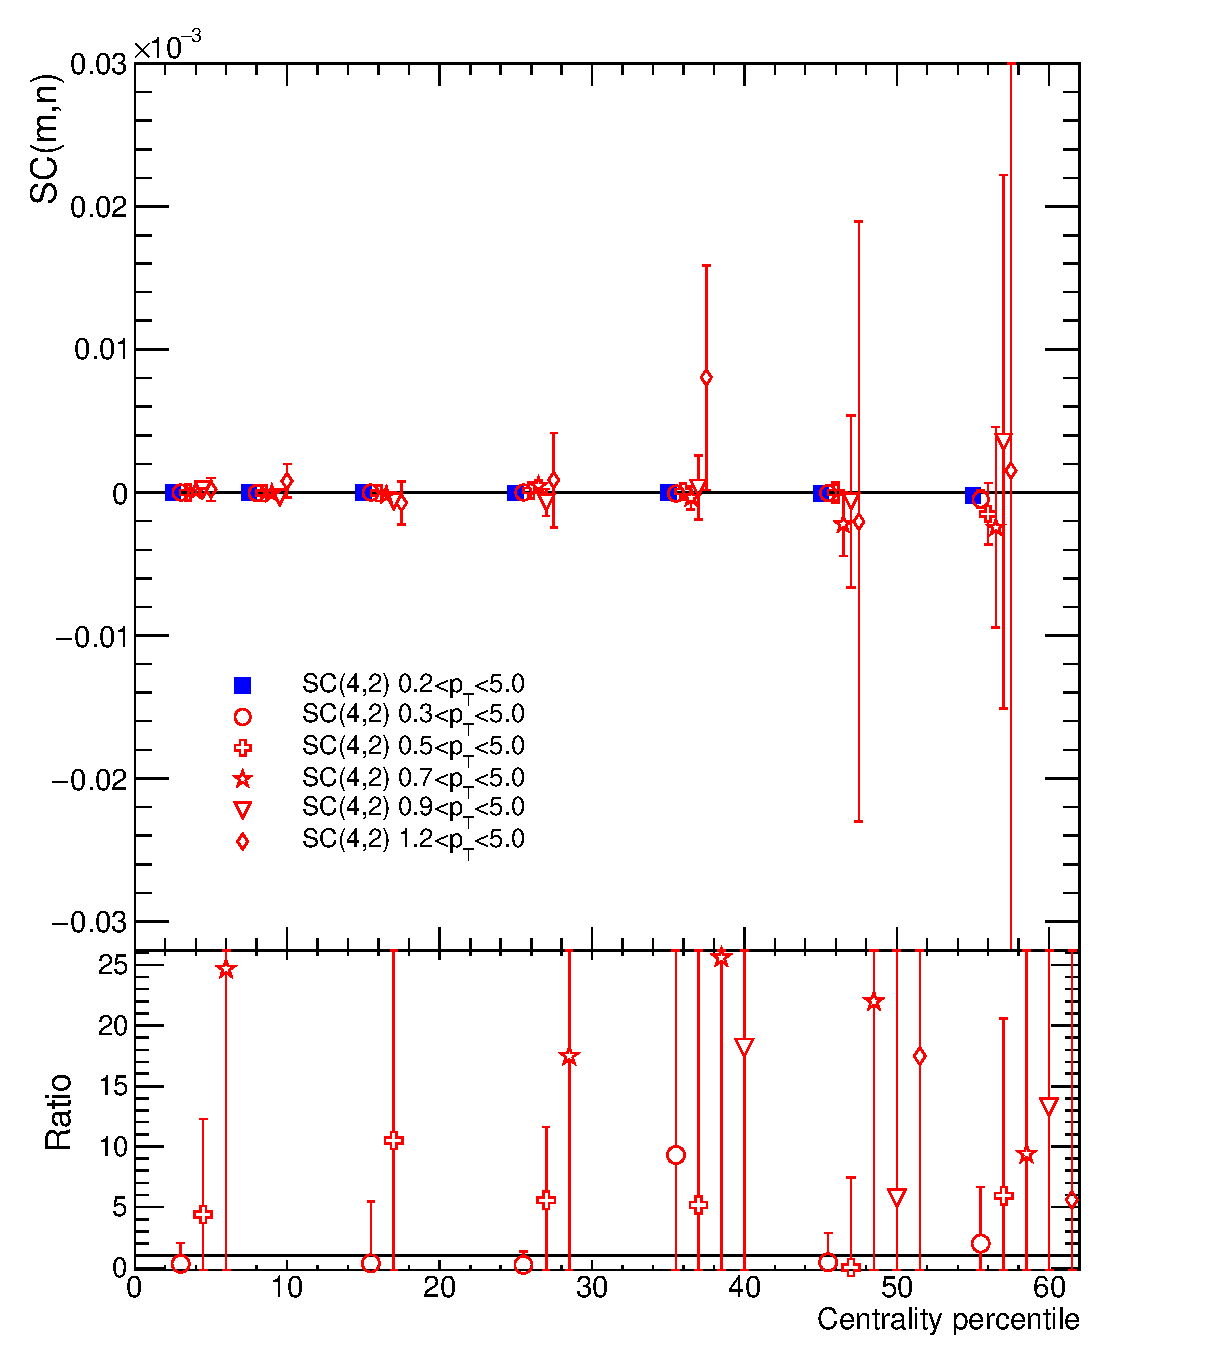
\includegraphics{figures/figs_results/SC_Comparison_SC42_HIJING_ptdep}}
        \caption{Result of SC(3,2) and SC(4,2) with HIJING simulations. Defaults($0.2 < p_T < 5.0GeV/c$) are drawn as full square with blue color, and different minimum cut conditions are listed in legend. A small shifts along the x axis were applied for better visibility}
        \label{fig:results_HIJING}
        \end{center}   
     \end{figure}



 \subsection{Model Comparison}

Various models have been used in this study. The {HIJING} model~\cite{Wang:1991hta,Gyulassy:1994ew} was used to estimate the strength of non-flow correlations (typically few-particle correlations insensitive to the collision geometry) as described in previous section. 

The $SC(m,n)$ from hydrodynamic prediction with pQCD, where the initial energy density profiles are calculated using a next-to-leading order perturbative-QCD+saturation model~\cite{Paatelainen:2012at,Paatelainen:2013eea} + various shared viscosity $\eta/s$ parameterizations were performed by H. Niemi \cite{Niemi:2015qia}. The subsequent spacetime evolution is described by relativistic dissipative fluid dynamics with different parametrizations for the temperature dependence of the shear viscosity to entropy density ratio $\eta/s(T)$. Each of the $\eta/s(T)$ parametrizations is adjusted to reproduce the measured $v_n$ from central to mid-peripheral collisions. 

 The fluid hydrodynamic predictions with the different parameterizations for the temperature dependence of the shear viscosity to entropy ratio $\eta/s(T)$ are shown shown in Figure.\ref{figs:sc} as dashed line. Roughly the hydrodynamic calculations capture qualitatively the centrality dependence, but not quantitively. Both $SC(3,2)$ with data and hydrodynamics have negative values for all centralities, while $SC(4,2)$ results have positive values over all measured centralities. However, there is no single centrality for which a given $\eta/s(T)$ parameterization describes both $SC(3,2)$ and $SC(4,2)$ simultaneously. On the other hand, the same hydrodynamic calculations capture the centrality dependence of the individual $v_n$ quantitively~\cite{Eskola:2015uda}.

$NSC(3,2)$ and $NSC(4,2)$ are also compared to the same model on the right in Fig.~\ref{figs:sc}. 
While $NSC(3,2)$ does not show sensitivity to  different $\eta/s(T)$ parameterizations,  $NSC(4,2)$ exhibit much better sensitivity
than $NSC(3,2)$ observable and the individual flow harmonics~\cite{Niemi:2015qia}.
These findings indicate that $NSC(3,2)$ observable is sensitive mainly to the initial conditions, while $NSC(4,2)$ observable is sensitive to both the initial conditions and the system properties, which is consistent with the prediction from~\cite{Niemi:2012aj}.

However, the sign of $NSC(3,2)$ is positive in the models in 0-10\% central collisions while it is negative in data.
In the most central collisions the anisotropies originate mainly from fluctuations, i.e.\ the initial ellipsoidal geometry characteristic for mid-central collisions plays little role in this regime. Hence this observation will help to understand the fluctuations in initial conditions better.

$NSC(4,2)$ observable shows better sensitivity for different $\eta/s(T)$ parameterizations, i.e. medium property but the model cannot describe the centrality dependence nor the absolute values. These observed distinct discrepancies between data and models might indicate that the current understanding of initial conditions used in the model need to be revisited
to further constrain the $\eta/s(T)$, considering the difficulties on separating the role of the $\eta/s$  from the initial condition to the final state particle anisotropies~\cite{Romatschke:2007mq,Shen:2011zc}.
Hence the use of $SC(m,n)$ and $NSC(m,n)$ can provide new constraints on the detailed modeling of the initial-state condition and the fluctuations of the medium created in heavy ion collisions and the better constraints on the initial-state conditions will certainly improve the uncertainties of determining $\eta/s(T)$.



 The normalized $SC(m,n)$ were compared to MC-Glauber using wounded nucleon (WN) and binary collisions (BC) weights models to check linear and non-linear response from initial geometry.  Assuming only linear response $v_n \propto \epsilon_n$, we expect that the normalized $SC(m,n)$ evaluated in coordinate space are able to capture the measurement of centrality dependence of normalized $SC(m,n)$ in the momentum space. In this case the correlation between the $n$th and $m$th order harmonics were estimated with calculation of $SC(m,n)$ in the coordinate space as define as 
 
 \begin{equation}
SC(m,n)_{\epsilon}/\langle \epsilon_n^2 \rangle \langle \epsilon_m^2 \rangle  \equiv (\langle \epsilon_n^2 \epsilon_m^2 \rangle - \langle \epsilon_n^2 \rangle \langle \epsilon_m^2 \rangle) /  \langle \epsilon_n^2 \rangle \langle \epsilon_m^2 \rangle
\label{eq:sc_ecen}
\end{equation}

Where the $\epsilon_n$ is the $n$th order coordinate space anisotropy as defined in \cite{Alver:2010gr}. Since there are two different scenarios of the MC-Glauber model, we tested with both wounded nucleon (WN) and binary collisions (BC) weights and results are shown in Fig.\ref{fig:results_ecen}. An increasing trend from central to peripheral collisions with different sign has been observed and there is a large deviation of $NSC(4,2)$ between ALICE data and MC-Glauber model. This deviation increase from central to peripheral collision regions and this might indicate the contribution of the non-linear response of initial condition though hydrodynamic evolution. Moreover, the MC-Glauber model with  $NSC(3,2)$ describes better the data  than $NSC(4,2)$,  because the  $NSC(3,2)$ appears to be sensitive only to initial conditions and not sensitive to hydrodynamic properties ($\eta/s$). 


	\begin{figure}[h]
		\begin{center}
        	\resizebox{0.45\columnwidth}{!}{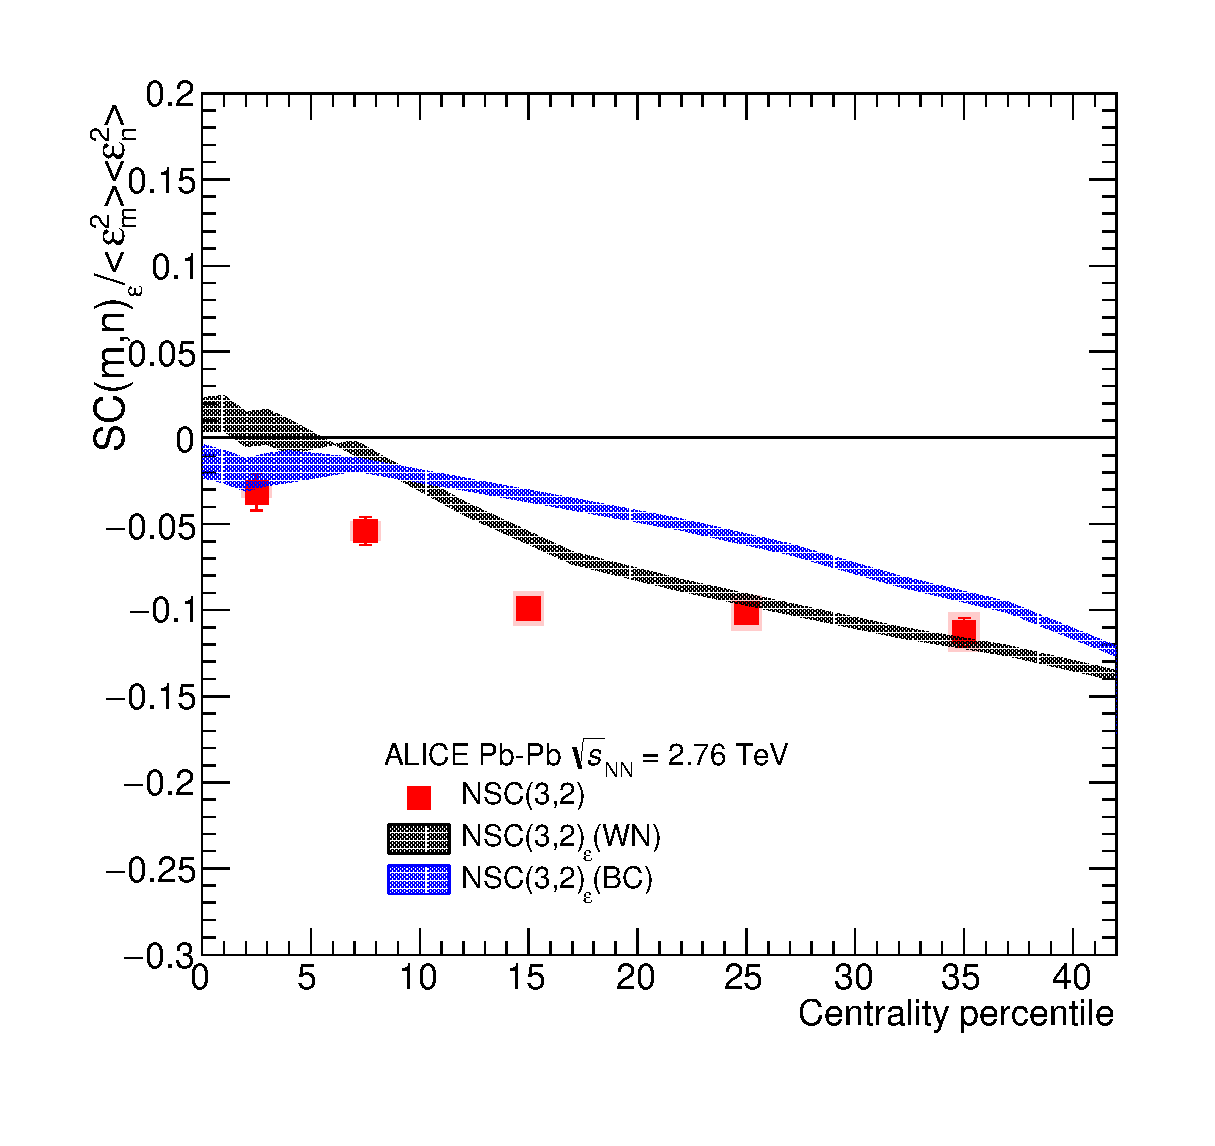
\includegraphics{figures/fig_ecen/SC_Comparison_ecen_BC_SC32}}
        	\resizebox{0.45\columnwidth}{!}{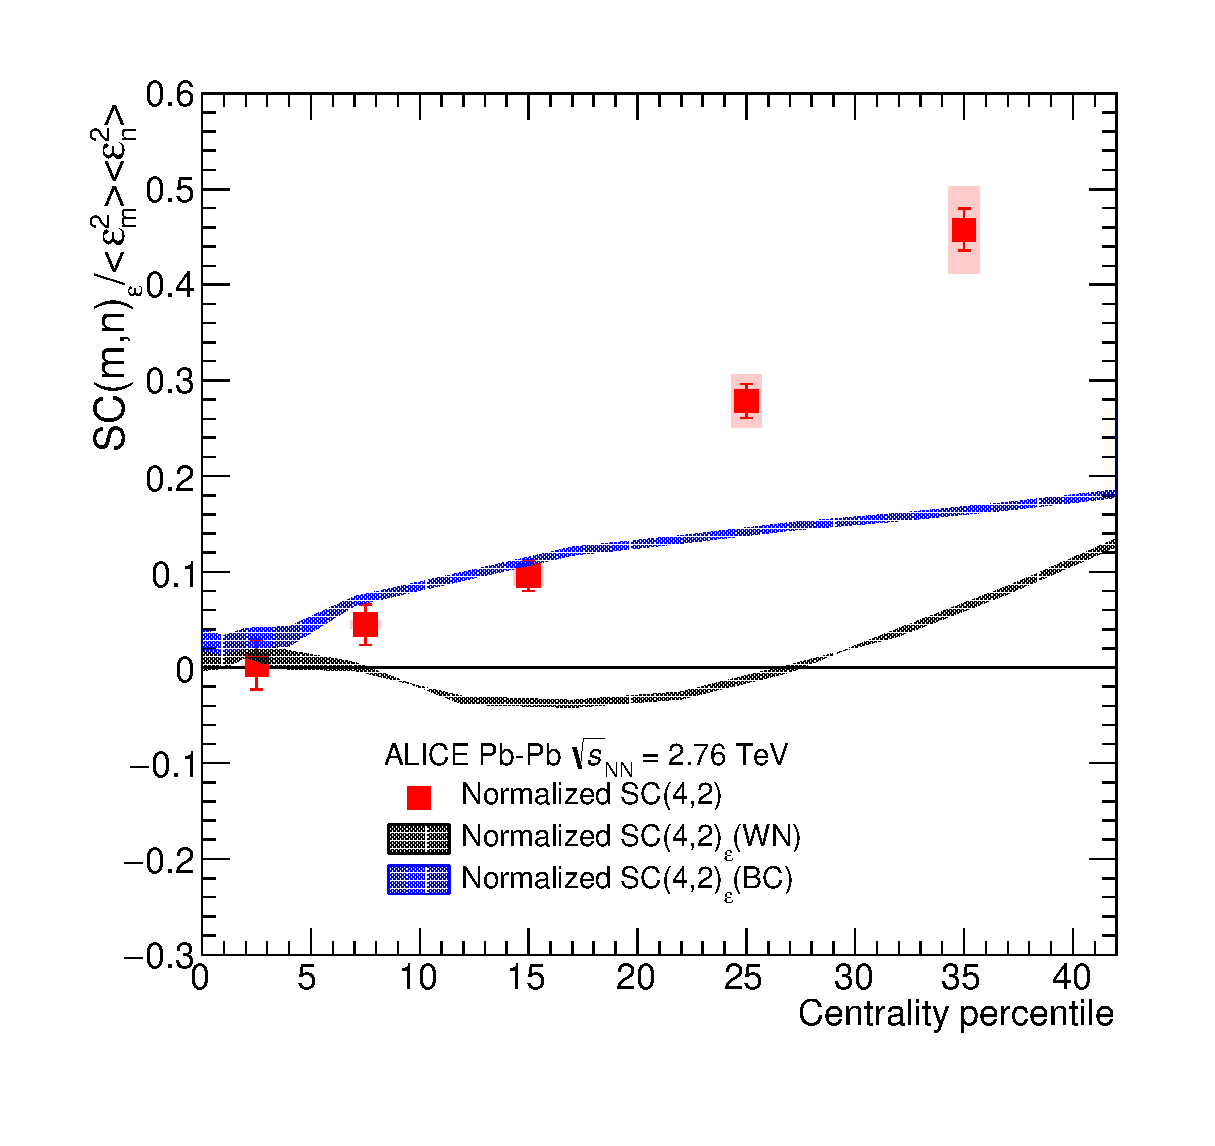
\includegraphics{figures/fig_ecen/SC_Comparison_ecen_BC_SC42}}
        \caption{Normalized $SC(m,n)$(red) with the comparison to MC-Glauber models using wonded nucleon (WN) and binary collisions (BC) wegiths.}
        \label{fig:results_ecen}
        \end{center}   
     \end{figure}



The $SC(m,n)$ with AMPT \cite{Zhang:1999bd,Lin:2000cx,Lin:2004en} simulation with various configurations was also tested. The configuration of AMPT are listed in Table.\ref{Tab:AMPTConf}. With changing configuration of AMPT simulations, we may estimate the effects of initial conditions and finite states effects. 

Even though thermalization could be achieved in collisions of very large nuclei and/or at extremely high energy, the dense matter created in heavy ion collisions may not achieve full thermal or chemical equilibrium as a result of its finite volume and energy. To address such non-equilibrium many-body dynamics, AMPT has been developed, which includes both initial partonic and final hadronic interactions and the transition between these two phases of matter.
For the initial conditions, the AMPT model uses the spatial and momentum distributions of hard minijet partons and soft strings from the HIJING model~\cite{Wang:1991hta,Gyulassy:1994ew}.
The AMPT model can be run in two main configurations, the default and the string melting model.
In the default version, partons are recombined with their parent strings when they stop interacting. The resulting strings are later converted into hadrons using the Lund string fragmentation model~\cite{Andersson:1986gw,NilssonAlmqvist:1986rx}. In the string melting version,  all the excited strings that are not projectile and target nucleons not experiencing any interactions are converted to partons according to the flavor and spin structures of their valence quarks. The advantage of this choice is that the AMPT model with string melting reduces to HIJING results in the absence of partonic and hadronic interactions as these partons would then find each other as closest partners at the same freeze-out time and thus coalesce back to the original hadron. In the AMPT model with string melting, the initial strings are melted into partons whose interactions are described by the ZPC parton cascade model~\cite{Zhang:1997ej}. These partons are then combined into the final-state hadrons via a quark coalescence model.  \cite{Lin:2005br}

In both configurations, the dynamics of the subsequent hadronic matter is described by a hadronic cascade based on a Relativistic Transport (ART) model~\cite{Li:2001xh} which also includes resonance decays.
The third version presented in this article is based on the string melting configuration, in which the hadronic rescattering phase is switched off to study its influence to the development of anisotropic flow.
The input parameters used in both configurations are: $\alpha_s = 0.33$, a partonic cross-section of 1.5~mb, while the Lund string fragmentation parameters were set to $\alpha = 0.5$ and $b = 0.9$~GeV$^{-2}$. 
Even though the string melting version of AMPT~\cite{Lin:2001zk,Lin:2004en} reasonably reproduces particle yields, $p_T$ spectra, and $v_2$ of low-$p_T$ pions and kaons in central and mid-central Au-Au collisions at $200$~GeV and Pb-Pb collisions at $2.76$~TeV~\cite{Lin:2014tya}, it was seen clearly in the recent study~\cite{Adam:2016nfo} that it fails to quantitatively reproduce the measurements. It turns out that the radial flow in AMPT is 25\% lower than the measured value at the LHC, which indicates that the unrealistically low radial flow in AMPT is responsible for the quantitative disagreement. The detail configurations on AMPT settings used for this article and the comparisons of $p_T$ differential $v_{n}$ for pions, kaons and protons to the data can be found in \cite{Adam:2016nfo}.






\begin{table}[!h]
\begin{center}
\begin{tabular}{c|c|c}
\hline 
Setting		    & String Melting    & Rescattering  \\  \hline  \hline
AMPT Default  & OFF     & ON        \\ \hline
AMPT String melting  & ON      &  ON        \\ \hline 
AMPT String melting w/o hadronic rescattering  & ON      & OFF         \\ \hline
\label{Tab:AMPTConf}
\end{tabular}
\caption{Configurations of AMPT simulation dataset which correspond to ALICE LHC10h data with Pb+Pb $\sqrt{S_{NN}}=2.76$TeV}
\end{center}
\end{table}


	\begin{figure}[!p]
		\begin{center}
        	\resizebox{0.48\columnwidth}{!}{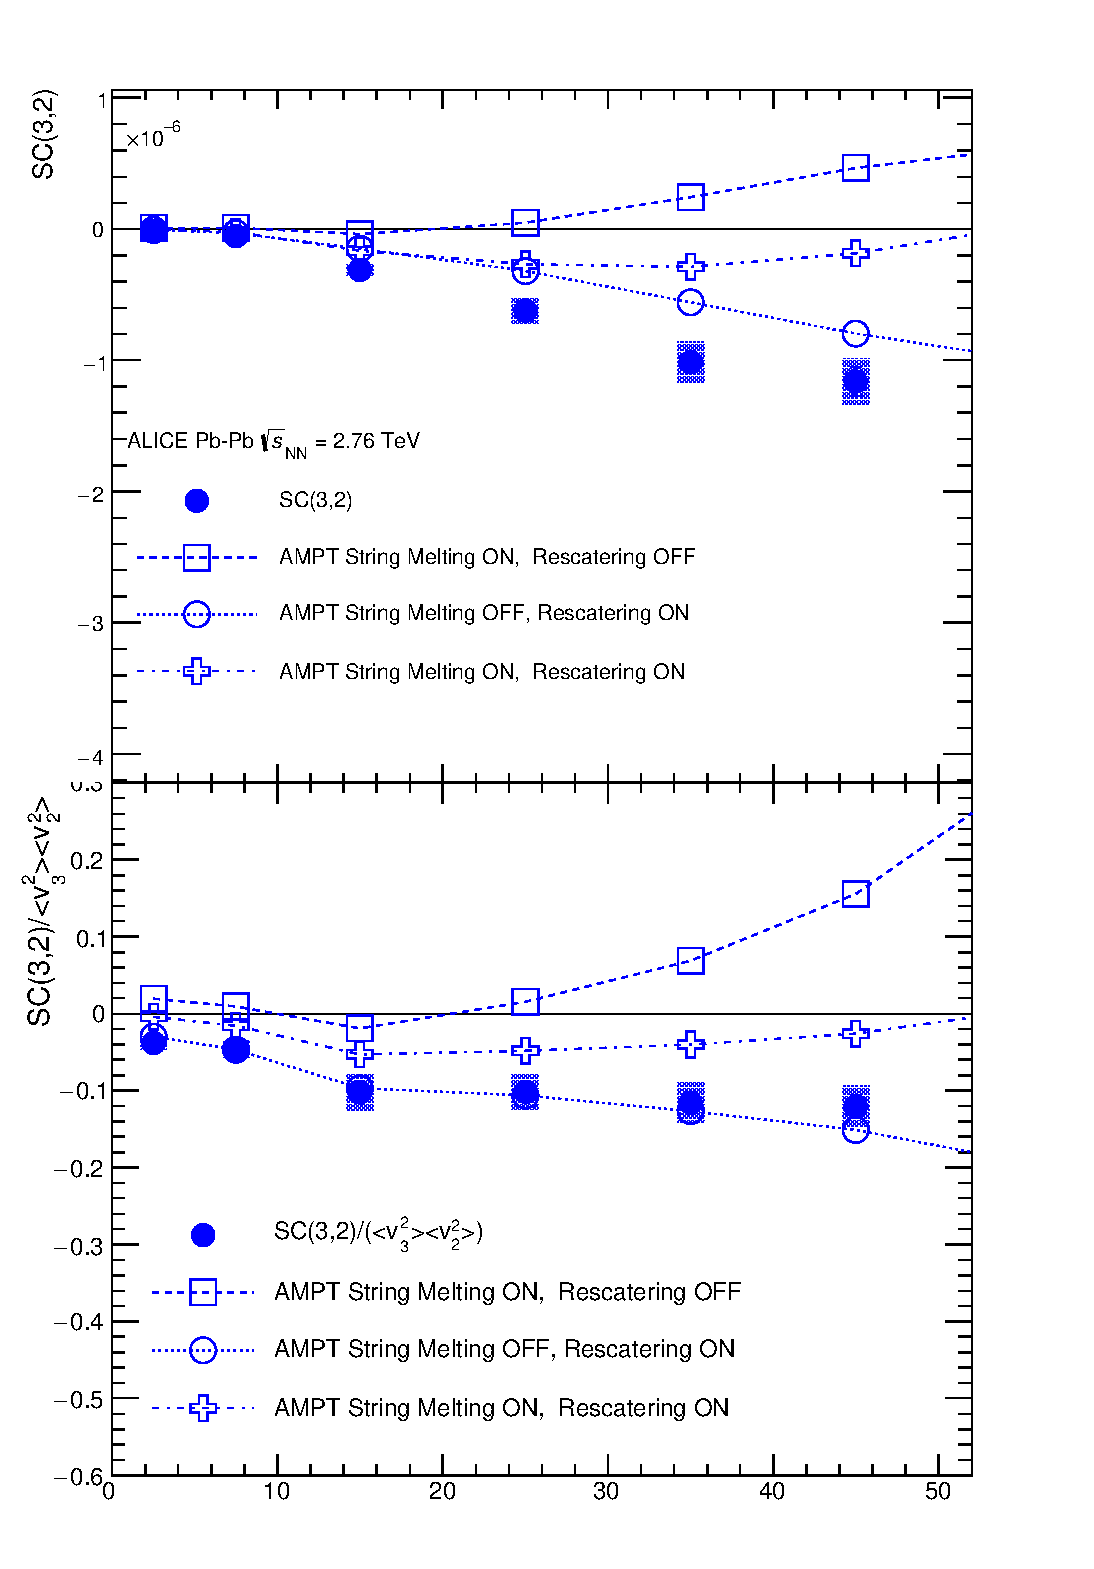
\includegraphics{figures/figs_results/fig3_QConly_ModelComparison_SC32_ampt.eps}}
        	\resizebox{0.48\columnwidth}{!}{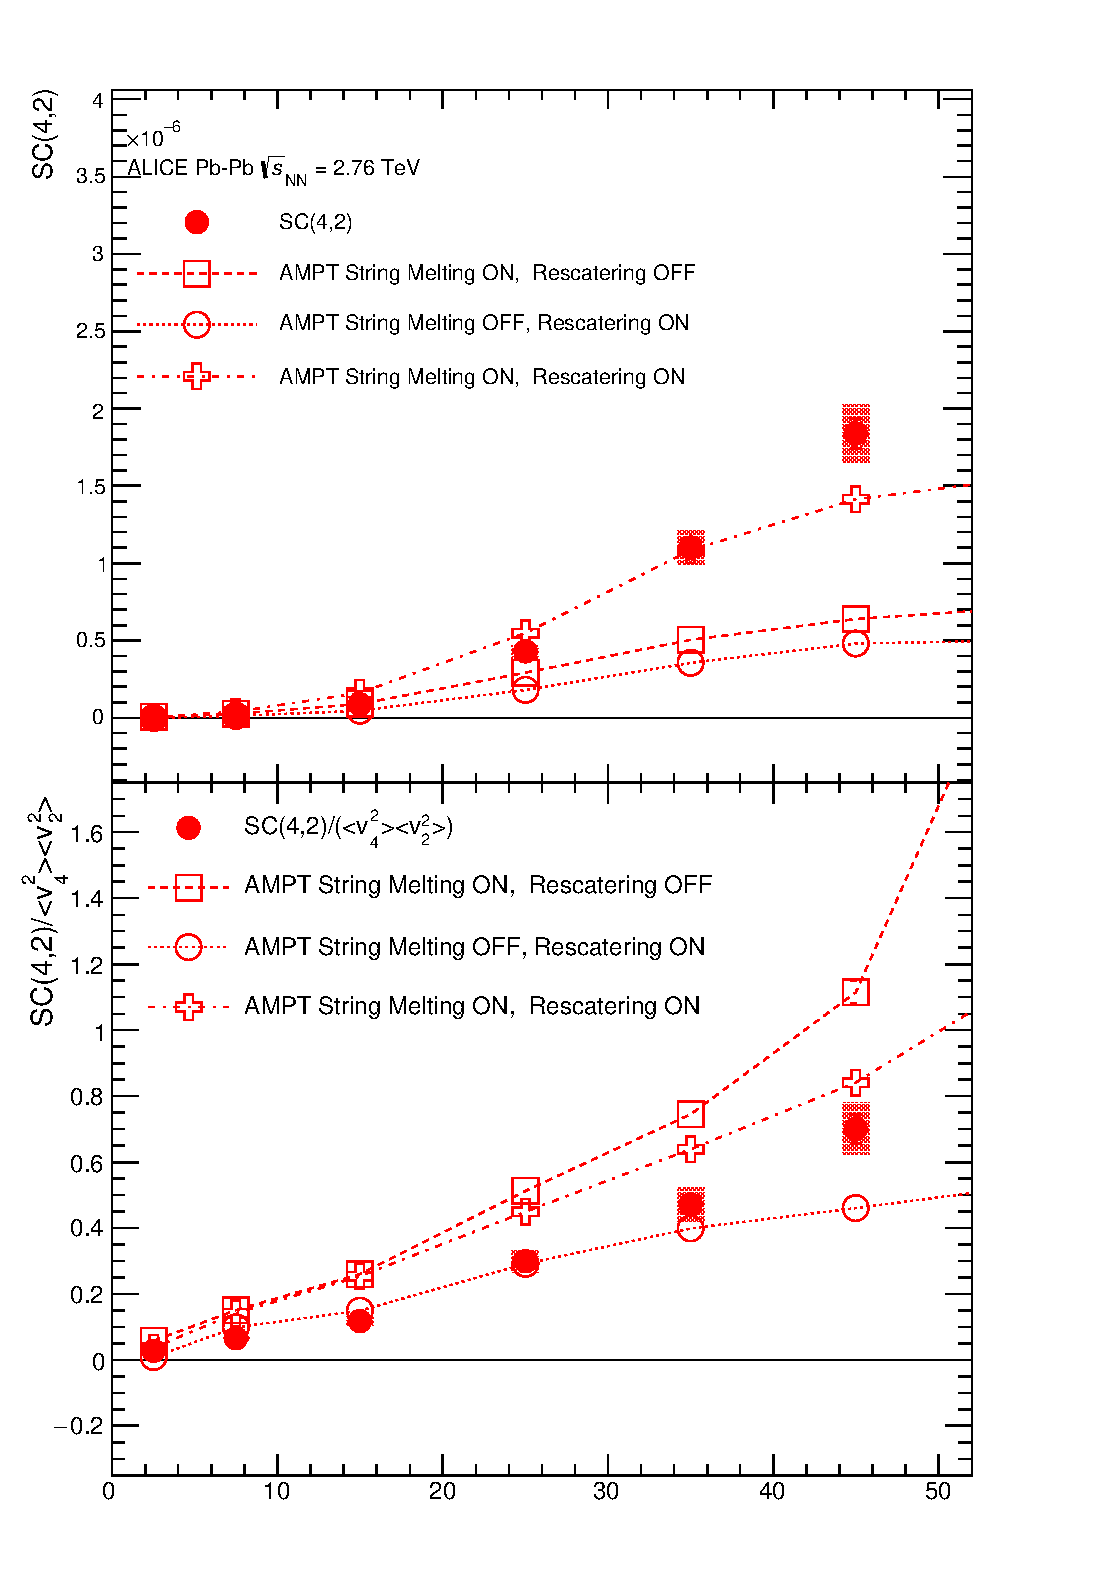
\includegraphics{figures/figs_results/fig3_QConly_ModelComparison_SC42_ampt.eps}}
        \caption{Result of  $SC(3,2)$ and $SC(4,2)$ with LHC10h data and comparison to various AMPT simulations with different settings.  The upper figures are the result of $SC(m,n)$ and the lower figures are the result of normalized $SC(m,n)$}
        \label{AMPTcomLowSC}
        \end{center}   
     \end{figure}

The results of comparison to AMPT are shown in Fig.\ref{AMPTcomLowSC}. As for $SC(3,2)$, neither of the settings can describe the data and somewhat the setting with the default AMPT model follows the trend of the data closest. The same setting can describe NSC(3,2) fairly well and also the sign of NSC(3,2) is well reproduced by this setting while all the hydrodynamic calculations in this article failed to describe the sign of the observable in most central collisions.

Interestingly the string melting AMPT model can't capture the data well where the strength of the correlation is weaker than the default model. The third version based on the string melting configuration with the hadronic rescattering phase off is also shown to study its influence. This late hadronic rescattering stage makes both $SC(3,2)$ and $NSC(3,2)$ stronger in the string melting AMPT model but it is not enough to describe the data.

Further we investigated why the default AMPT model can describe $NSC(3,2)$ fairly well but underestimates $SC(3,2)$. By taking the differences in the individual flow harmonics ($v_2$ and $v_2$) between the model and data into account, we was able to recover the data. The discrepancy in $SC(3,2)$ can be explained by the overestimated individual $v_n$ values reported in \cite{Adam:2016nfo} in all the centrality ranges. 

In case of $SC(4,2)$, the string melting AMPT model can fairly describe the data while the default model underestimates it.
$NSC(4,2)$ is slightly overestimated by the same setting which can describe $SC(4,2)$ but the default AMPT model can describe the data better.
The influence of the hadronic rescattering phase for $NSC(4,2)$ is opposite to other observables ($SC(3,2)$, $NSC(3,2)$ and $SC(4,2)$), where the hadronic rescattering make $NSC(4,2)$ slightly smaller.
It should be noted that the better agreement for $SC(m,n)$ should not be overemphasized since there are discrepancies in the individual $v_n$ between AMPT and data as it was demonstrated for $SC(3,2)$.
Hence the simultaneous description of $SC(m,n)$ and $NSC(m,n)$ should give better constrains to the parameters in AMPT.



	\begin{figure}[!p]
		\begin{center}
        	\resizebox{0.48\columnwidth}{!}{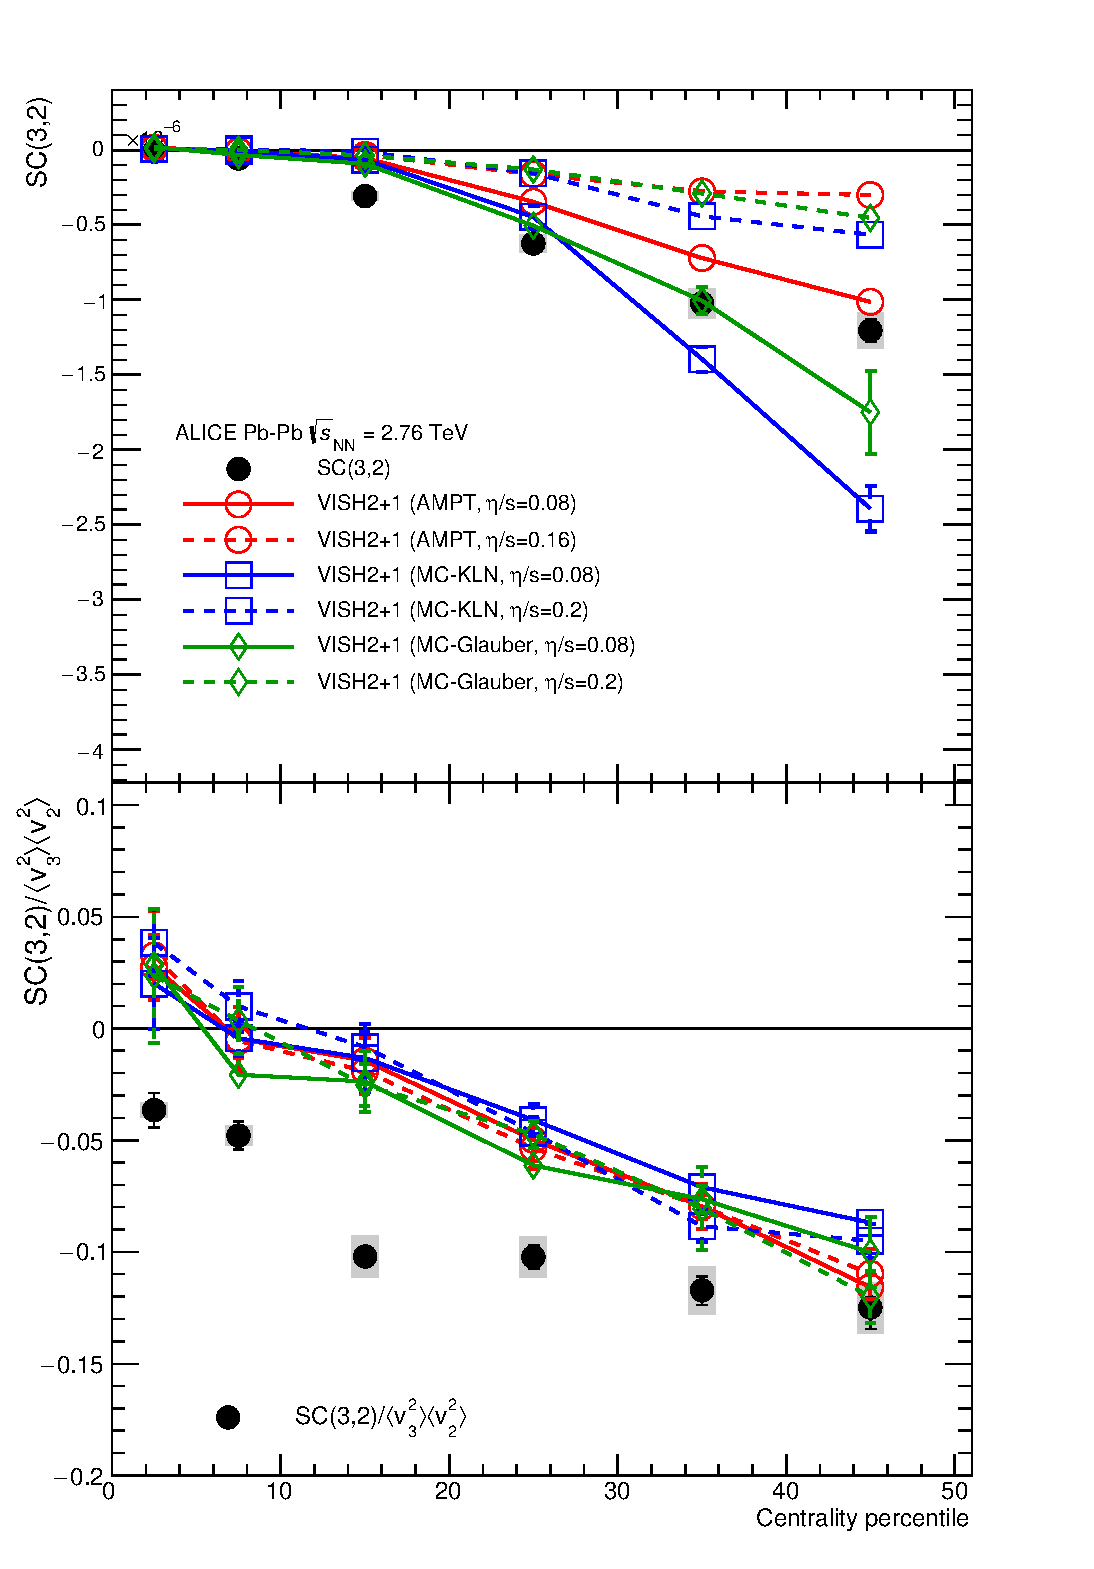
\includegraphics{figures/figs_results/fig3_QConly_ModelComparison_SC32_vish.eps}}
        	\resizebox{0.48\columnwidth}{!}{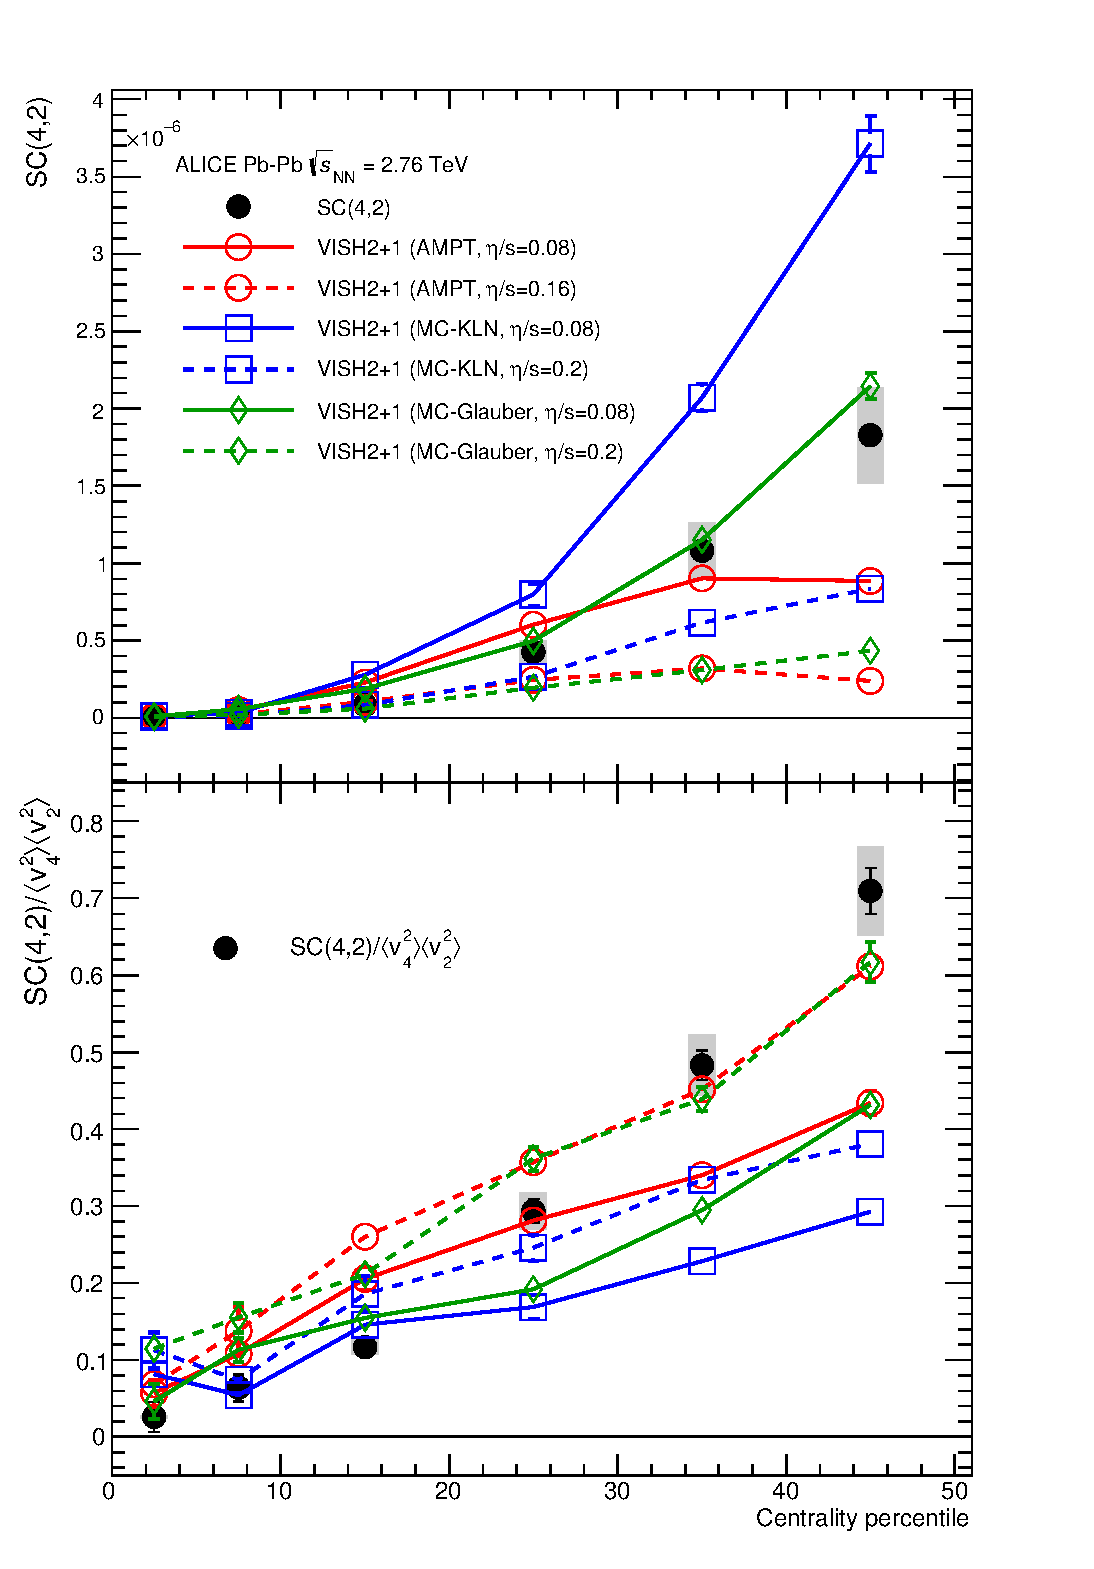
\includegraphics{figures/figs_results/fig3_QConly_ModelComparison_SC42_vish.eps}}
        \caption{Result of  $SC(3,2)$(left) and $SC(4,2)$(right) with LHC10h data and various VISH2+1 calculation with different settings. The three initial conditions from AMPT, KLN, and Glauber simulations are drawn as a different color. Furthermore, the hydrodynamic properties of $\eta/s$ are shown as line style, the small share viscosity ($\eta/s$=0.08) are shown as solid line, and large share viscosity ($\eta/s$=0.2 for KLN and Glauber, 0.16 for AMPT) is drawn as dashed line. Upper figures are the result of $SC(m,n)$ and lower figures are results of normalized $SC(m,n)$}
        \label{vish21}
        \end{center}   
     \end{figure}


  The comparison to VISH2+1 calculation are shown in Fig.\ref{vish21}. The VISH2+1~\cite{Zhu:2016puf} is an event-by-event theoretical framework model for relativistic heavy-ion collision based on (2+1)-dimensional viscous hydrodynamics which describes both the QGP fluid and the highly dissipative and even off-equilibrium late hadronic stage with fluid-dynamics. With well tuned transport coefficients, decoupling temperature  and some well-chosen initial conditions (like {AMPT}~\cite{Xu:2016hmp,Bhalerao:2015iya,Pang:2012he} etc.), it could fit many related soft hadron data, such as the $p_T$ spectra and different flow harmonics at RHIC and the LHC~\cite{Qiu:2011hf, Shen:2010uy, Shen:2011eg, Bhalerao:2015iya}.
Three different initial conditions ({MC-Glauber}, {MC-KLN} and {AMPT}) along with different constant $\eta/s$ parametrizations are used in the model. 
Traditionally, the Glauber model constructs the initial entropy density of the QGP fireball from a mixture of the wounded nucleon and binary collision density profiles~\cite{Kolb:2000sd}, and the {KLN} model assumes the initial entropy density is proportional to the initial gluon density calculated from the corresponding $k_T$ factorization formula~\cite{Kharzeev:2000ph}. In the Monte-Carlo versions ({MC-Glauber} and {MC-KLN})~\cite{Miller:2007ri,Drescher:2006ca,Hirano:2009ah}, additional initial state fluctuations are introduced through the position fluctuations of individual nucleons inside the colliding nuclei. For the {AMPT} initial conditions~\cite{Bhalerao:2015iya,Pang:2012he,Xu:2016hmp}, the fluctuating energy density profiles are constructed from the energy decompositions of individual partons, which fluctuate in both momentum and position space. Compared with the {MC-Glauber} and {MC-KLN} initial conditions, the additional Gaussian smearing parameter in the {AMPT} initial conditions makes the typical initial fluctuation scales changeable which gives rise to non-vanishing initial local flow velocities~\cite{Pang:2012he}. 

As shown in the Fig.\ref{vish21},  all the models with the large share viscosity regardless of the initial conditions ($\eta/s$=0.2 for MC-KLN and MC-Glauber initial conditions and $\eta/s = 0.16$ for AMPT initial condition) failed to capture the centrality dependence of $SC(3,2)$ and $SC(4,2)$.  However, for the normalized case($NSC$), all the results with different parameters do not have much difference as like original $SC(m,n)$. It may suggest that the $\eta/s$ parametrization affects the single flow magnitude, (generally large share viscosity($\eta/s$) leads short mean free path($\lambda_{mfp}$) and it decreases the flow magnitudes) rather than affect on correlations between flow orders. 
And among the models with small shear viscosities ($\eta/s$=0.08), the one with the AMPT initial condition describes the data better both for $SC(3,2)$ and $SC(4,2)$ but they cannot describe the data quantitively for most of the centrality ranges.
As similarly as the above mentioned hydrodynamic calculations~\cite{Niemi:2015qia}, the sign of the $NSC(3,2)$ in these models is opposite to the data in 0-10\% central collisions. $NSC(3,2)$ don't show sensitivity to neither initial conditions nor $\eta/s$ parametrizations and cannot be described by these models quantitively.
However, for $NSC(4,2)$, it is sensitive both to initial conditions and $\eta/s$ parametrizations.
Even though $NSC(4,2)$ is flavoured both by AMPT initial condition with $\eta/s$=0.08 and MC-Galuber initial condition with $\eta/s$=0.20,
$SC(4,2)$ can be only described by smaller $\eta/s$ from AMPT and MC-Glauber initial conditions. Therefore the Galuber initial condition with $\eta/s$=0.20 model can be ruled out and we come to a conclusion based on the tested model parameters that $\eta/s$ should be small and AMPT initial condition is flavoured by the data.
  

\section{Higher order flow harmonics results}

In this section, we will present the results of the correlation between higher order flow harmonics up to 5th order. The results with q-Cumulants method (SP method) with $|\eta| < 0.8$, $0.2 < p_T < 5.0$GeV/$c$ from ALICE data are shown. The lower order $SC(m,n)$ are scaled down and drawn together as colored band for comparison.


	\begin{figure}[hp]
		\begin{center}
        	\resizebox{0.87\columnwidth}{!}{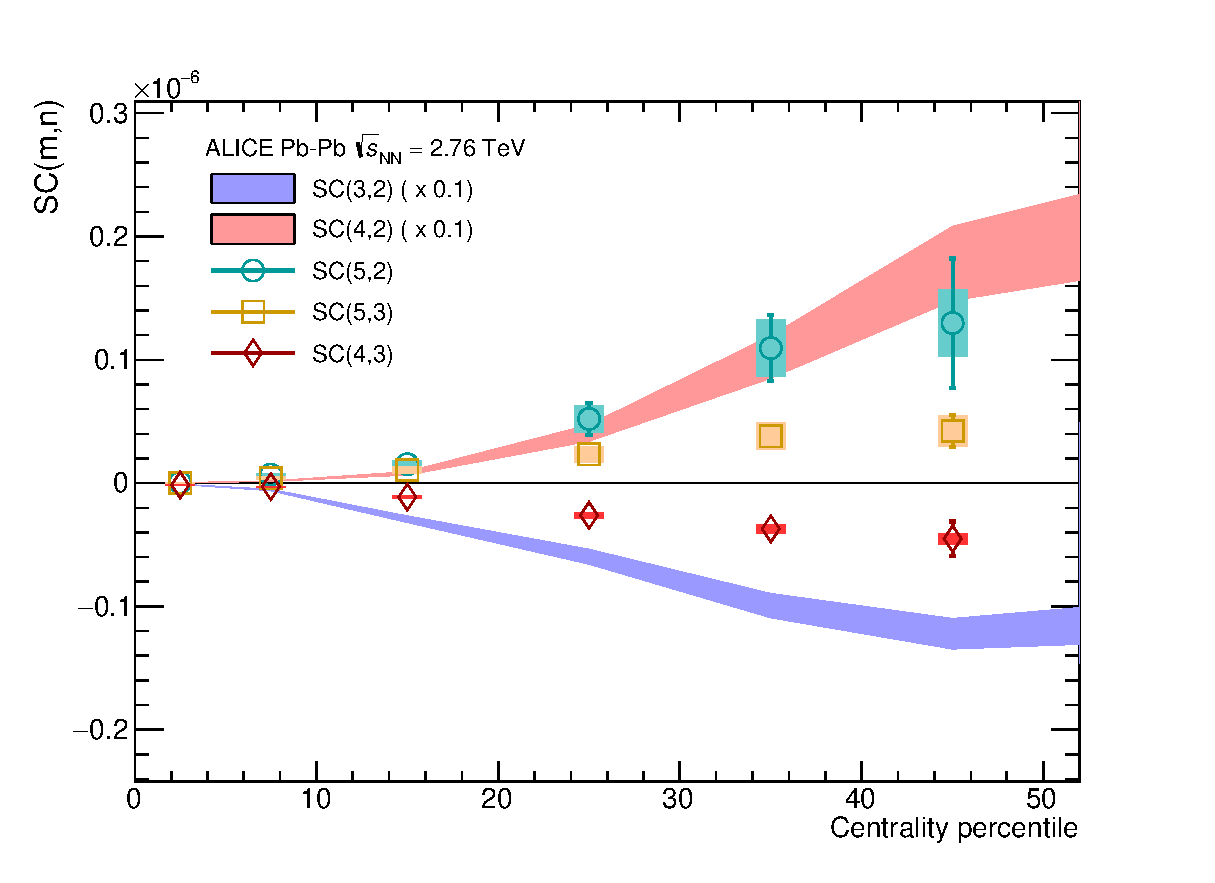
\includegraphics{figures/figs_results/fig2_QConly_higherSC}}
        	\resizebox{0.87\columnwidth}{!}{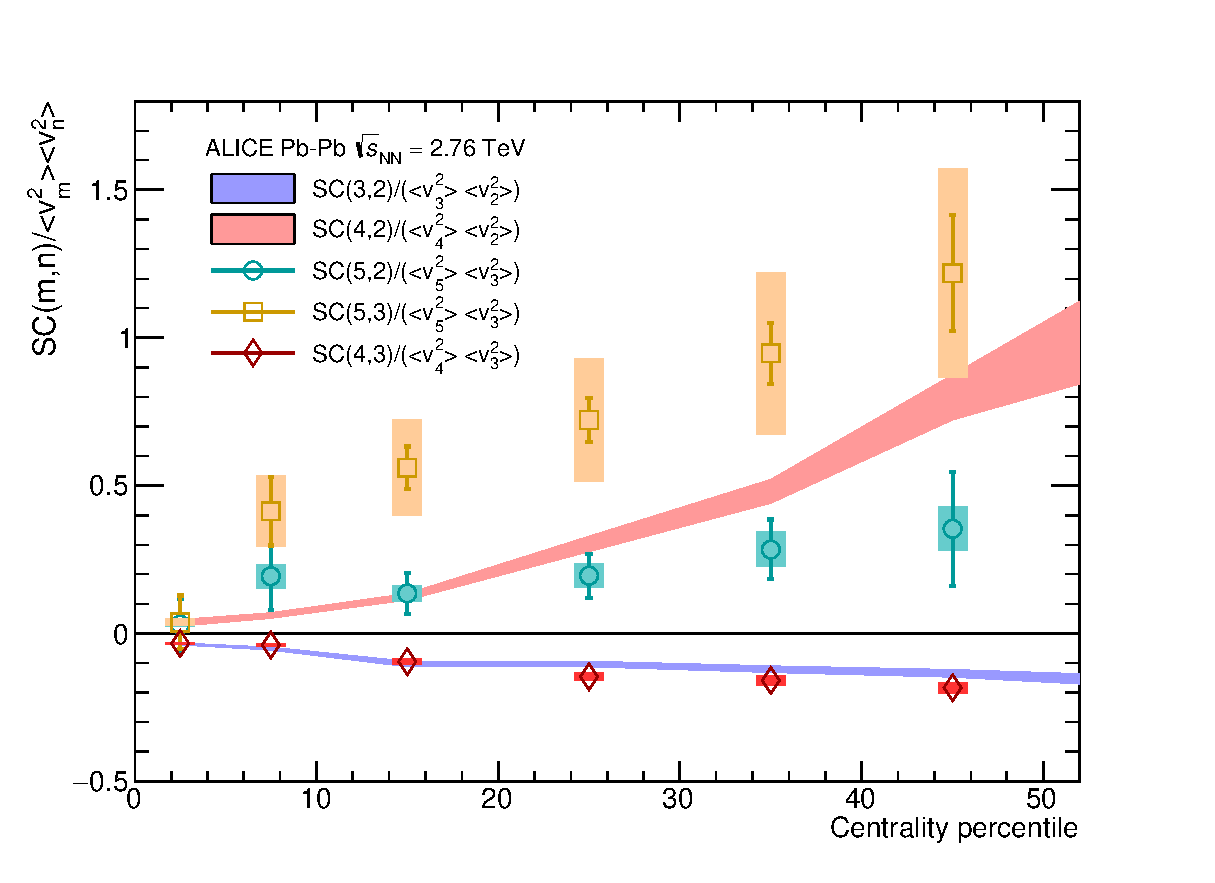
\includegraphics{figures/figs_results/fig2_QConly_higherNSC}}
        \caption{The result of $SC(m,n)$(upper figure) and $NSC(m,n)$(bottom figure) with higher order up to 5th flow harmonics with q-Cumulants method from ALICE Pb+Pb $\sqrt{S_{NN}}=2.76$TeV. Note that The lower order $SC(m,n)$ are scaled down. Both $SC(m,n)$ and $NSC(m,n)$ with lower orders are drawn as colored band and statistical and systematical errors were quadratically merged. }
        \label{fig:highersc}
        \end{center}   
     \end{figure}


As predicted as hydrodynamic calculation \cite{Bhalerao:2015jg} the correlation between $v_3^2$ and $v_4^2$ is negative and the others are positive. The correlation between higher harmonics ($v_3$ and $v_4$, $v_2$ and $v_5$, $v_3$ and $v_5$) become smaller for more central collisions, and it suggests that the correlation is likely due to the non-linear contributions of higher order flow harmonics like $v_4$ and $v_5$ \cite{PhysRevC.85.024908}. 

However, unlike $SC(m,n)$, $NSC(m,n)$ results with the higher order flow harmonics show almost same order of the correlation strength as the lower order flow harmonic correlations ($NSC(3,2)$ or $NSC(4,2)$). $NSC(4,3)$ is comparable to $NSC(3,2)$ and one finds that a hierarchy $NSC(5,3) > NSC(4,2) > NSC(5,2)$ holds for most of centrality ranges within the errors.
These results indicate that the lower oder harmonic correlations ($SC(3,2)$ and $SC(4,2)$) are larger than higher order harmonic correlations ($SC(4,3), SC(5,2)$, and $SC(5,3)$), not only because of the correlation strength itself but also the individual flow strength. 
$SC(5,2)$ is stronger than $SC(5,3)$, however as for $NSC$, the correlation between $v_5$ and $v_3$ is stronger than the correlation between $v_5$ and $v_2$. 


	\begin{figure}[h]
		\begin{center}
        	\resizebox{0.325\columnwidth}{!}{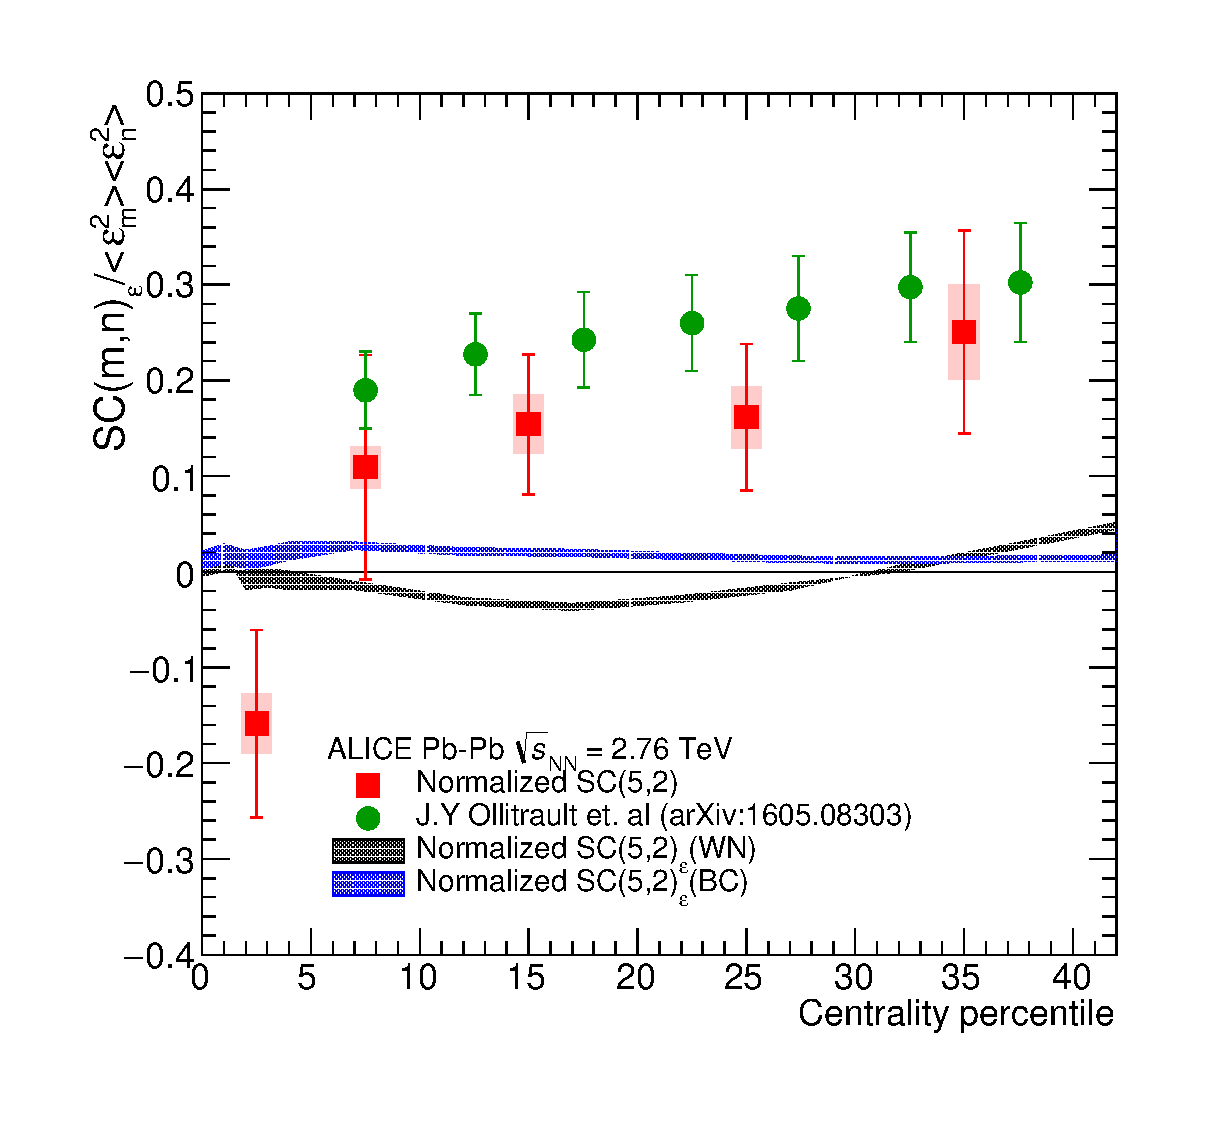
\includegraphics{figures/fig_ecen/SC_Comparison_ecen_BC_SC52}}
        	\resizebox{0.325\columnwidth}{!}{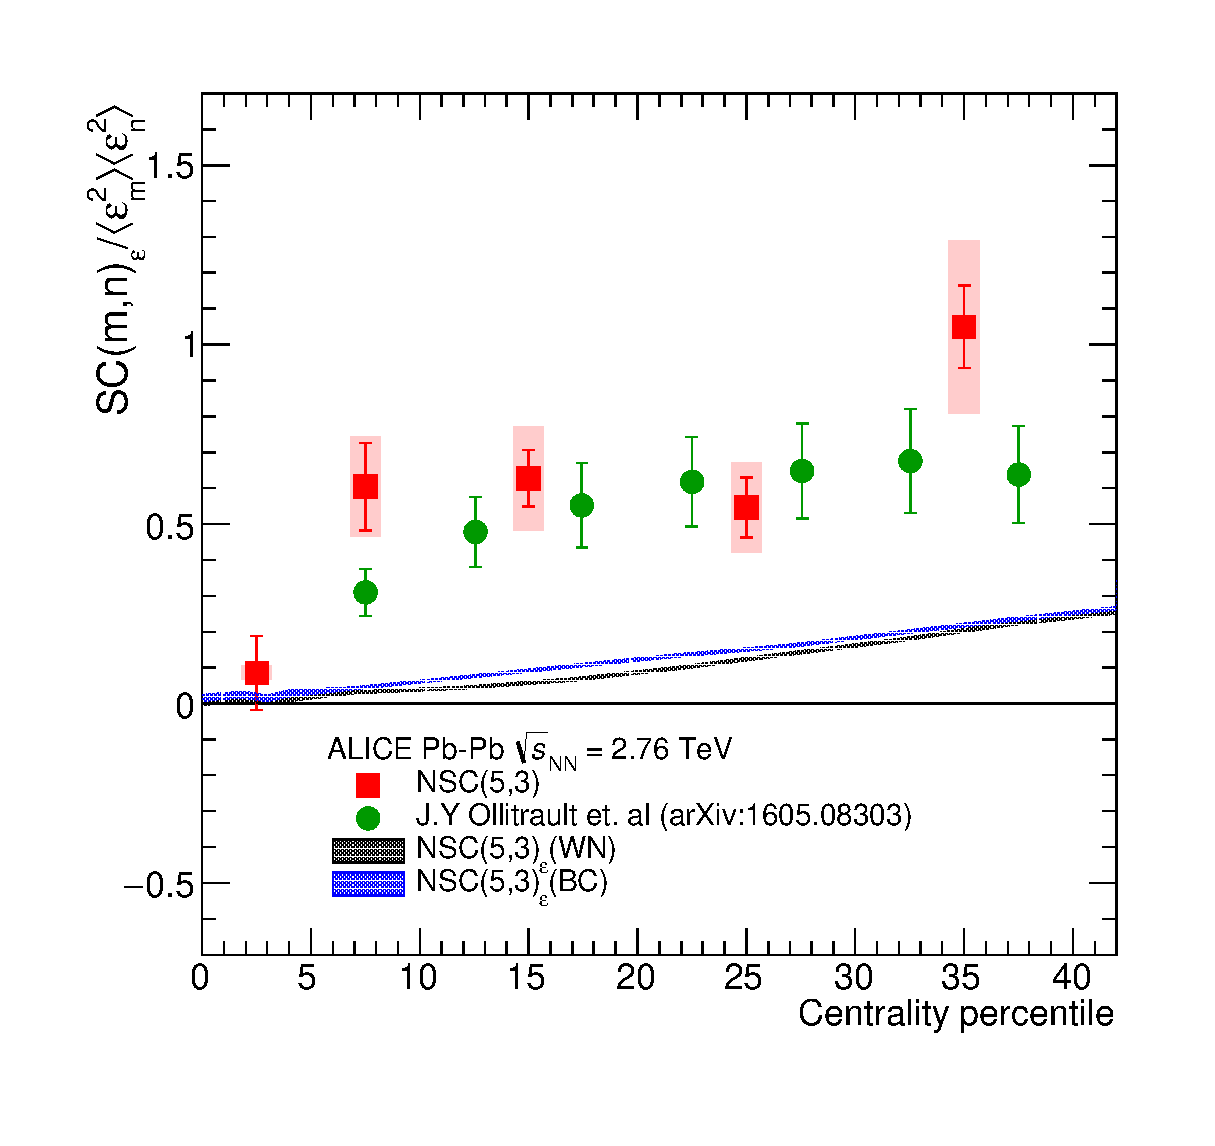
\includegraphics{figures/fig_ecen/SC_Comparison_ecen_BC_SC53}}
        	\resizebox{0.325\columnwidth}{!}{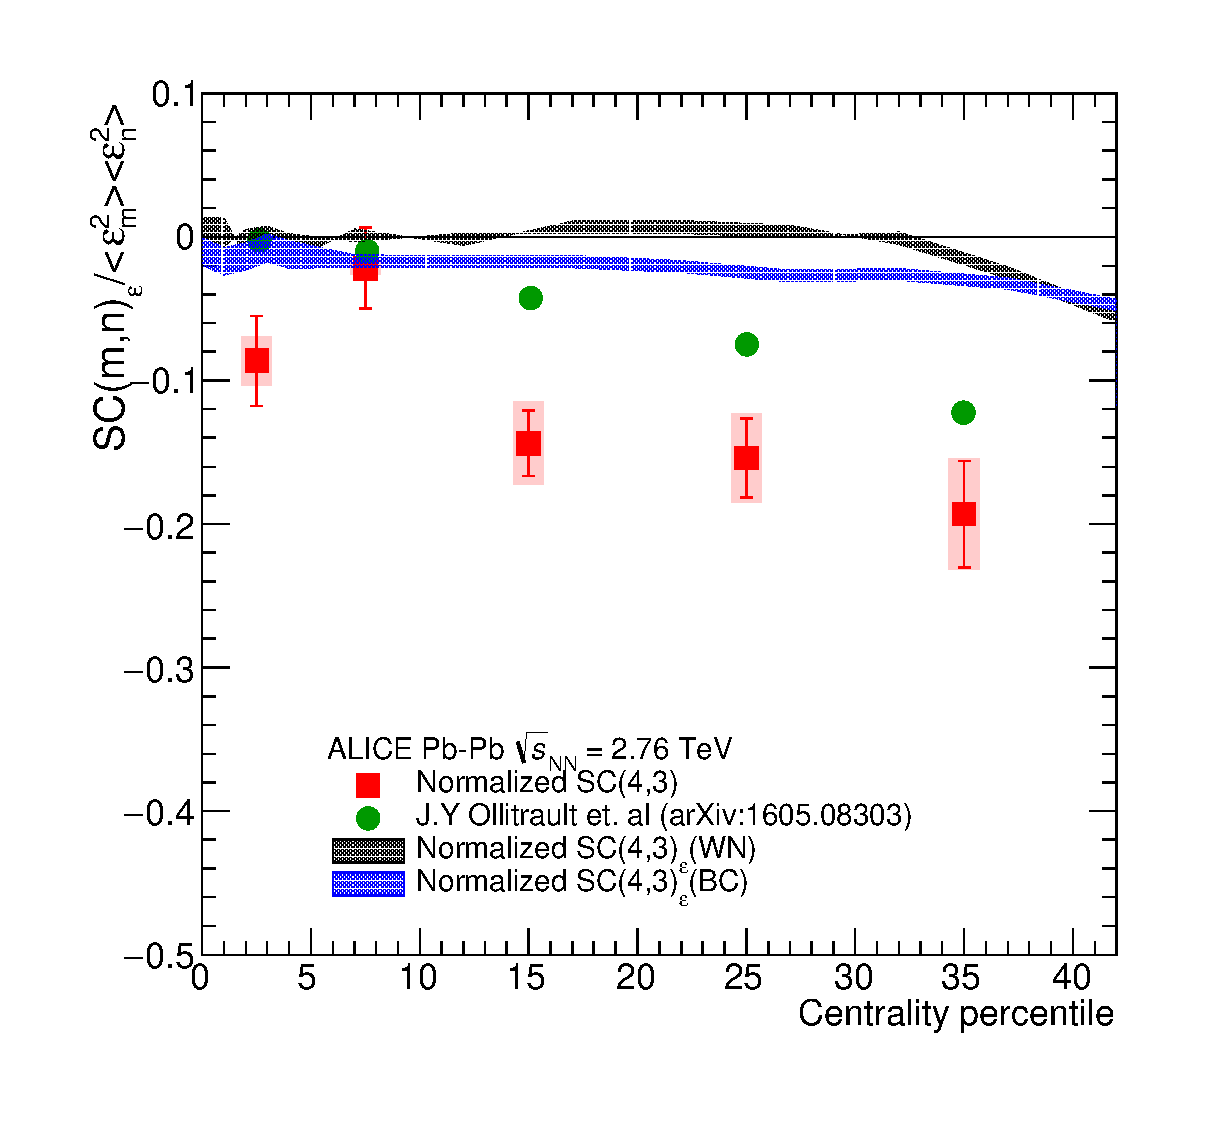
\includegraphics{figures/fig_ecen/SC_Comparison_ecen_BC_SC43}}
        \caption{Result of  higher order $NSC(m,n)$ and comparison to MC-Glauber models and prediction from J.Y Ollitraults\cite{Giacalone:2016afq}  }
        \label{fig_sc_higher:glauber}
        \end{center}   
     \end{figure}

 The $NSC(m,n)$ with higher order harmonics were compared to MC-Glauber to check the response (both linear and non-linear) of initial geometry. The $NSC(m,n)$ in coordinate space (as defined in Eq.\ref{eq:sc_ecen}) with both WN and BC weights were compared and shown in Fig.\ref{fig_sc_higher:glauber}. The large differences between MC-Glauber models (both WN and BC) and data shows that the correlation between flow harmonics can not be explained by only linear contribution of initial fluctuation. Also the prediction from J.Y Ollitraults from ALICE lower order $SC(m,n)$ and EP(Event Plane) correlation from ATLAS with few assumptions\cite{Giacalone:2016afq} were shown together as green marker in Fig.\ref{fig_sc_higher:glauber}. Although it predict better than any other existing theoretical models, however still have some deviation between data for $NSC(4,3)$ case.
 

	\begin{figure}[h]
		\begin{center}
        	\resizebox{0.325\columnwidth}{!}{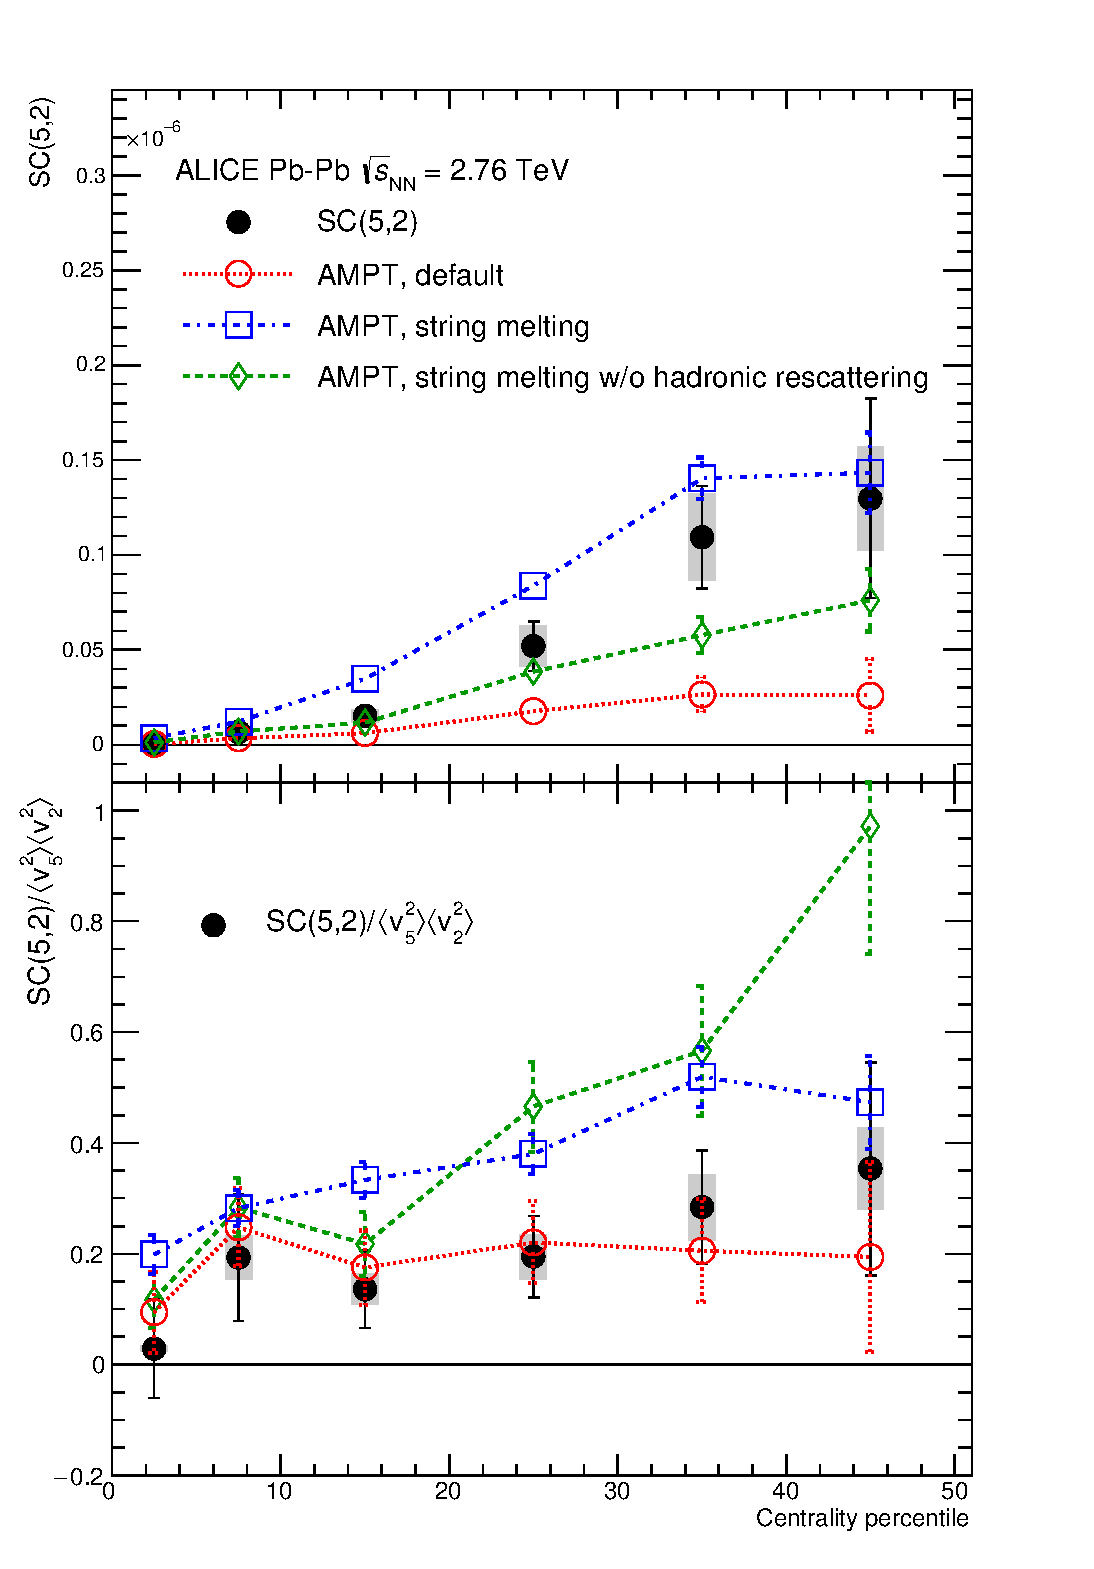
\includegraphics{figures/figs_results/fig3_QConly_ModelComparison_SC52_ampt.eps}}
        	\resizebox{0.325\columnwidth}{!}{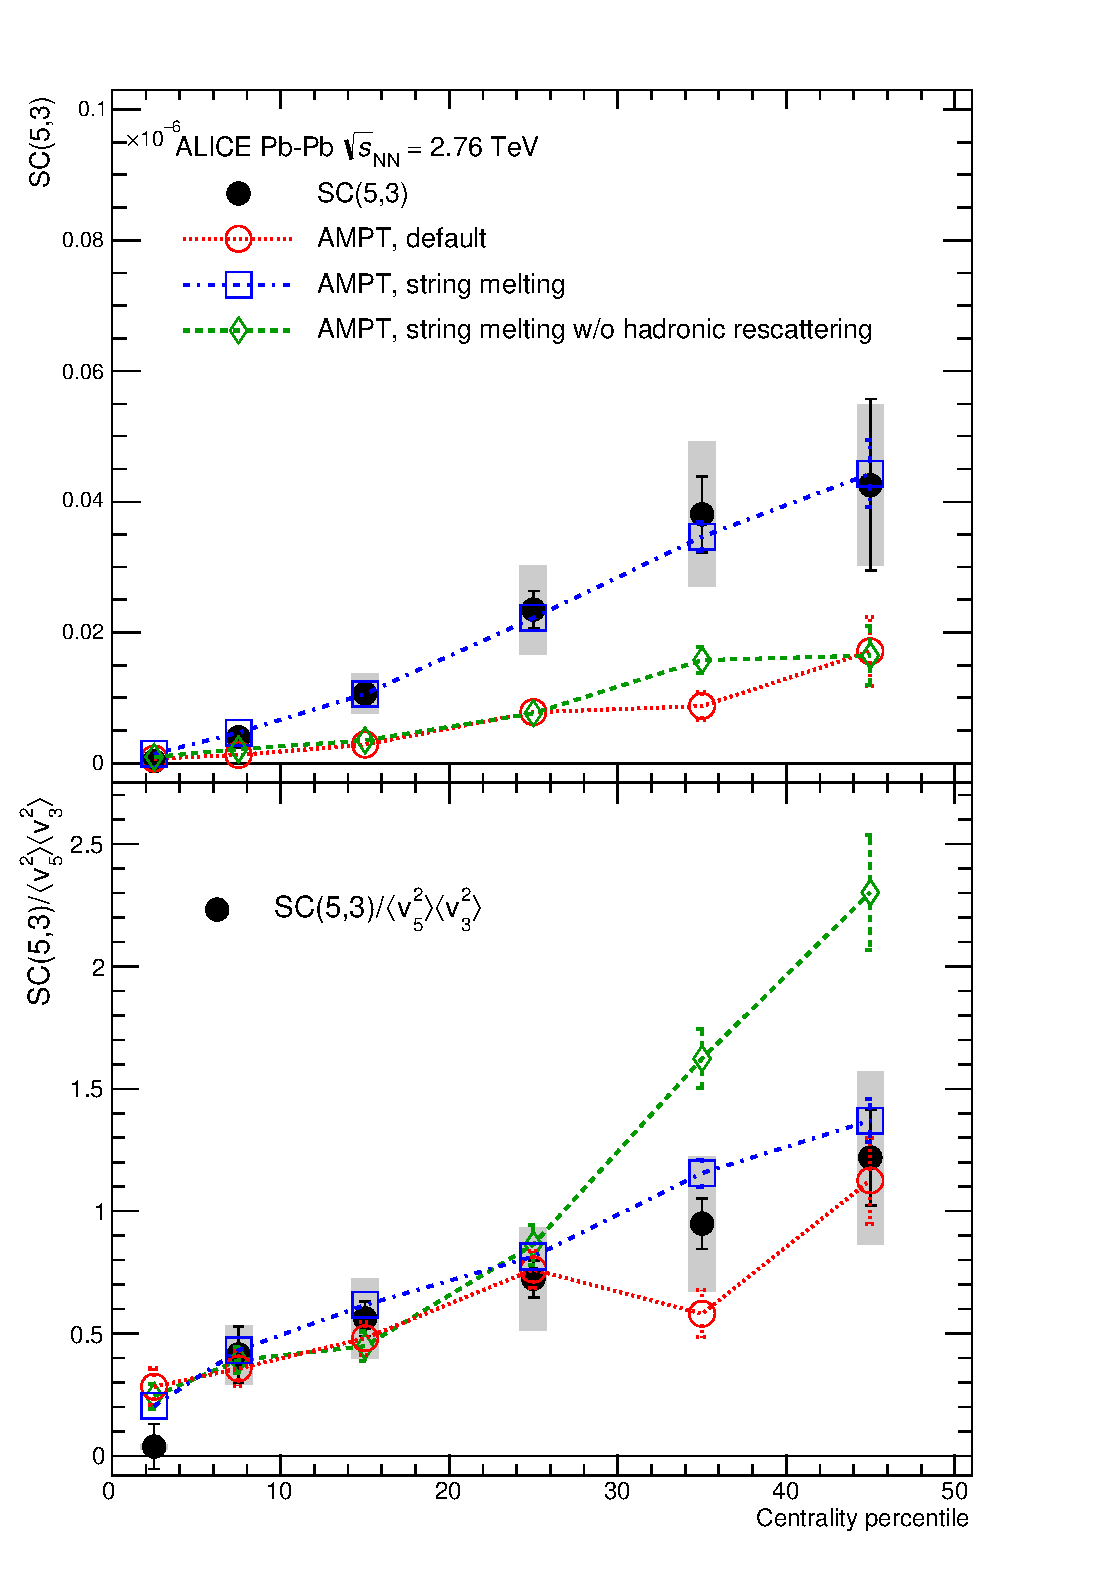
\includegraphics{figures/figs_results/fig3_QConly_ModelComparison_SC53_ampt.eps}}
        	\resizebox{0.325\columnwidth}{!}{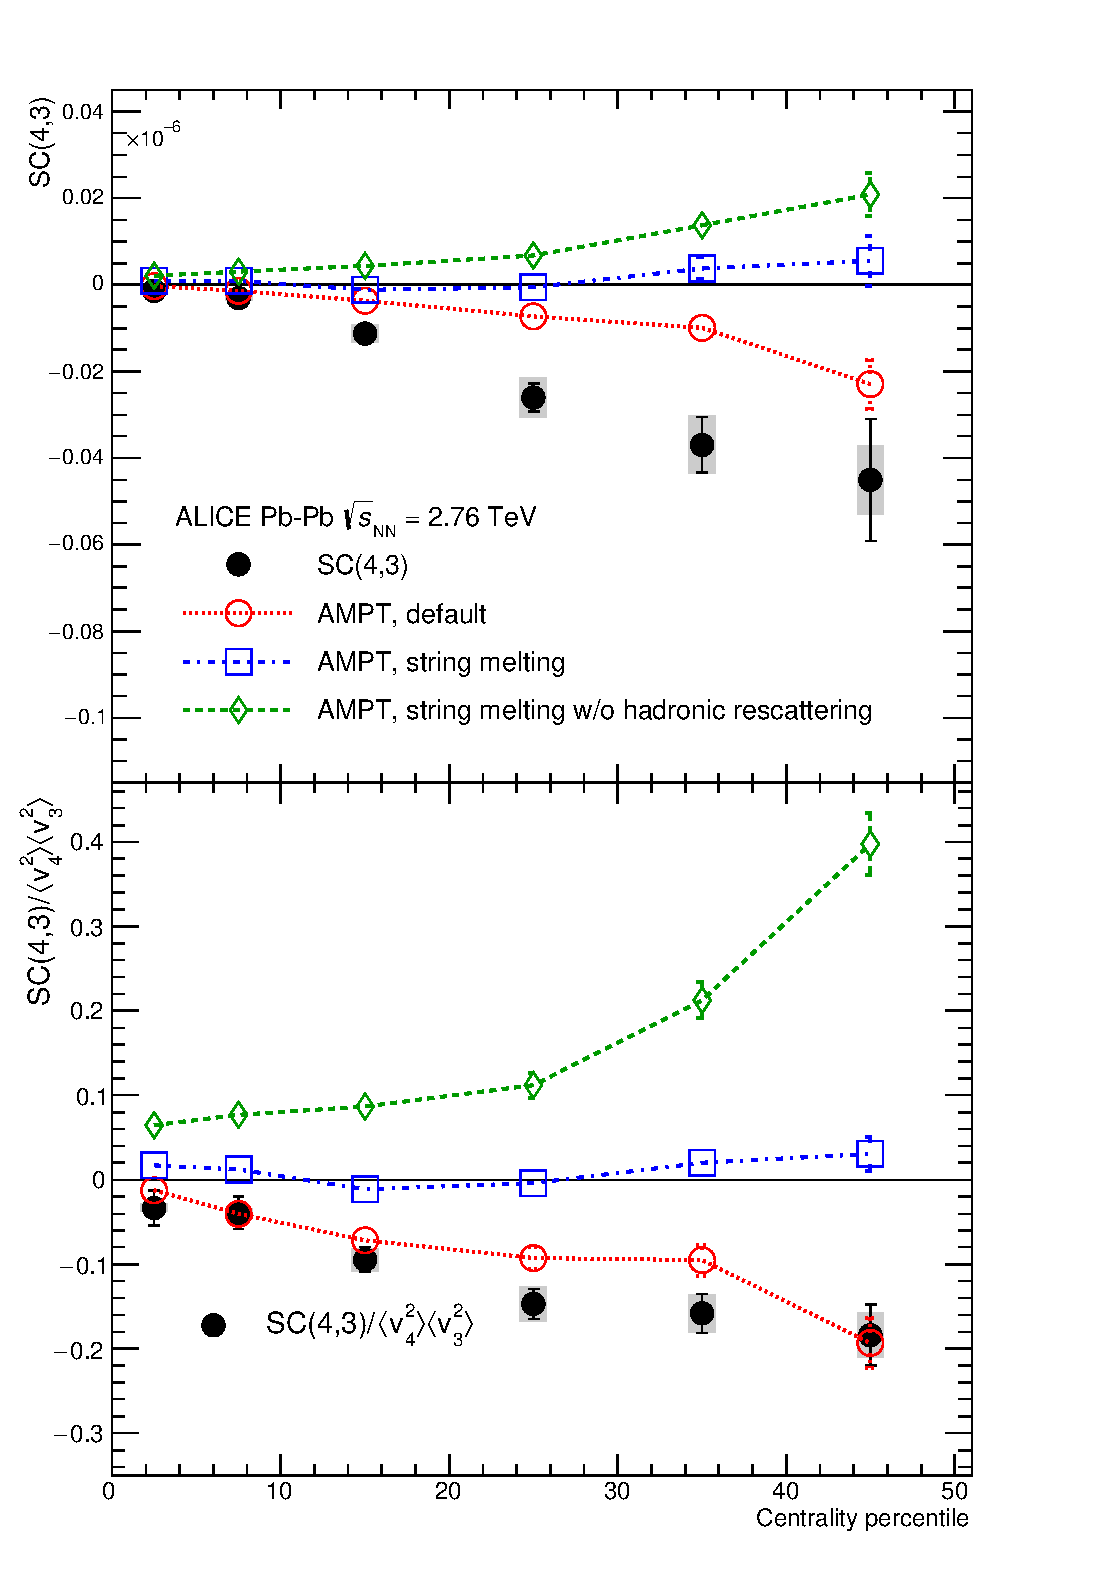
\includegraphics{figures/figs_results/fig3_QConly_ModelComparison_SC43_ampt.eps}}
        \caption{Result of  $SC(5,2)$, $SC(5,3)$ and $SC(4,3)$ and comparison to various AMPT simulations with different settings.  Upper figures are the results of $SC(m,n)$ and the lower figures are the results of $NSC(m,n)$}
        \label{AMPTcomhigh}
        \end{center}   
     \end{figure}
     
     
The extracted results  from particle level AMPT simulations in the same way as for the data are compared to the data in Fig.\ref{fig:AMPTcomhigh}.
The string melting AMPT model describes SC(5,2) and SC(5,3) well. The same setting describes only $NSC(5,3)$. However, it overestimates $NSC(5,2)$. 
However the default AMPT model can describe $NSC(5,3)$ and $NSC(5,2)$ fairly well as similarly as $NSC(3,2)$ and $NSC(4,2)$.
In case of $SC(4,3)$, neither of the settings can describe the data but the default AMPT model follows the data closest. 
The string melting AMPT model fails to describe $SC(4,3)$ and $NSC(4,3)$.
In summary, the default AMPT model describes the normalized SC (NSC$(m,n)$) from lower to higher order harmonic correlation while the string melting AMPT model overestimates $NSC(5,2)$ and 
underestimates (or very week correlations) $NSC(4,3)$. 
     

	\begin{figure}[h]
		\begin{center}
        	\resizebox{0.325\columnwidth}{!}{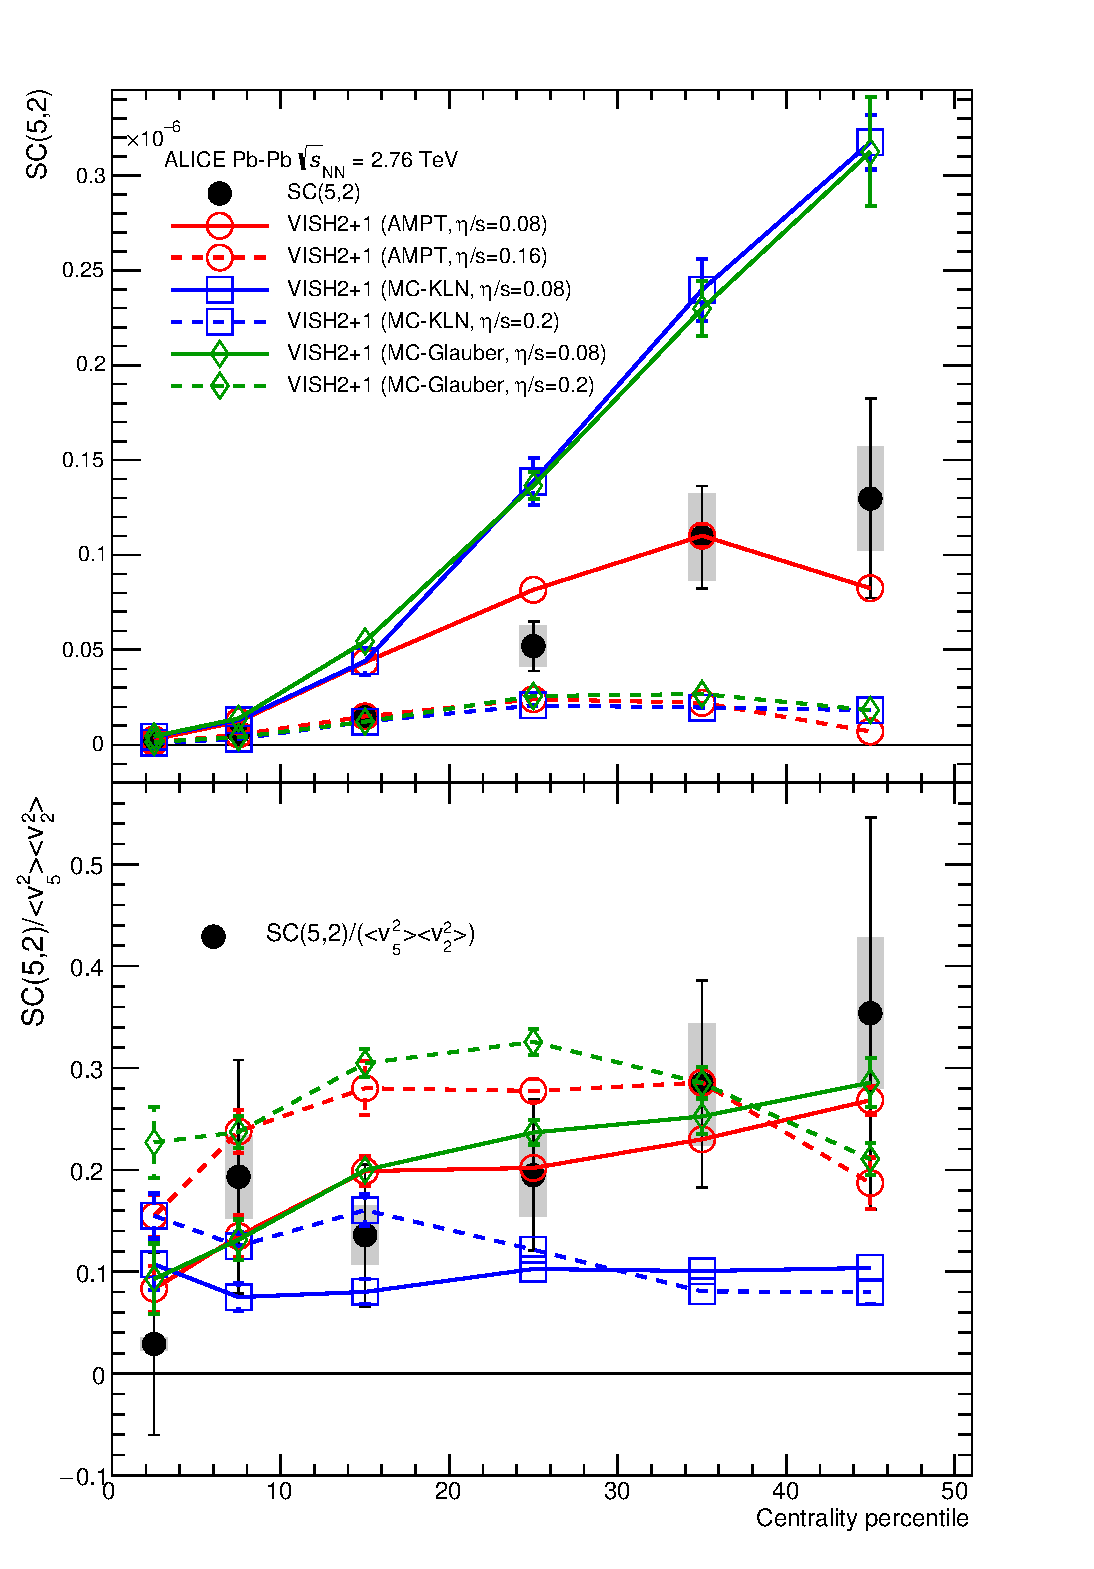
\includegraphics{figures/figs_results/fig3_QConly_ModelComparison_SC52_vish.eps}}
        	\resizebox{0.325\columnwidth}{!}{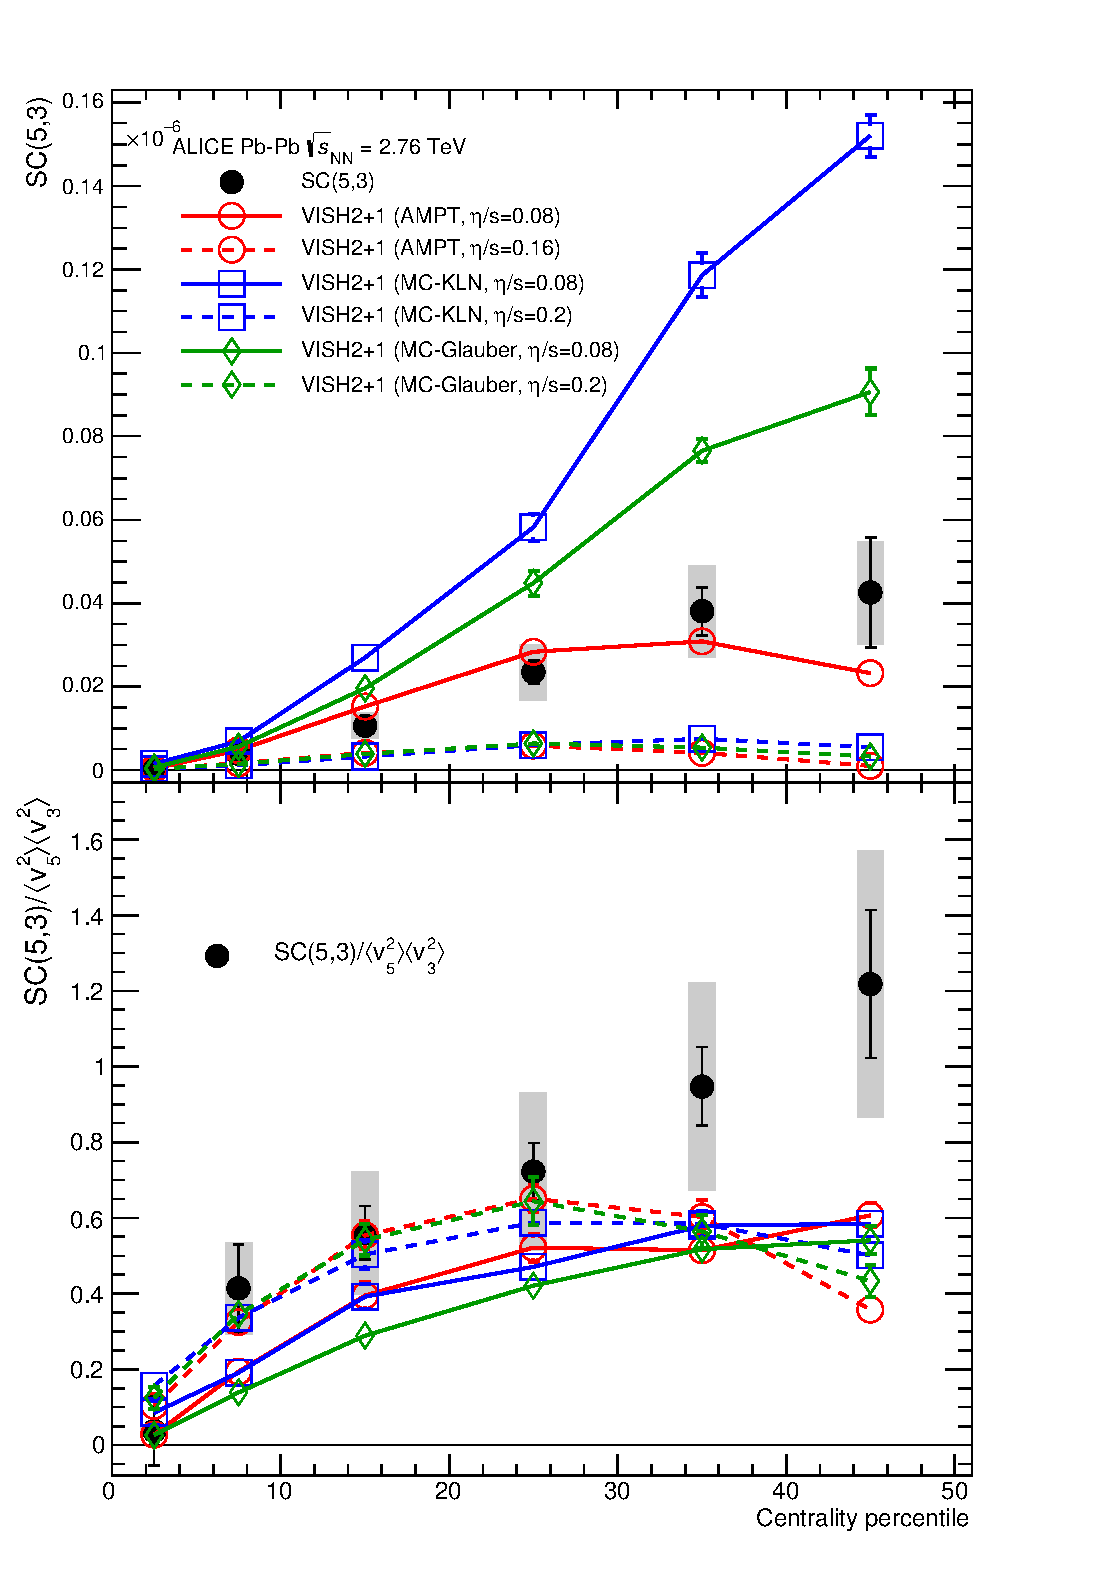
\includegraphics{figures/figs_results/fig3_QConly_ModelComparison_SC53_vish.eps}}
        	\resizebox{0.325\columnwidth}{!}{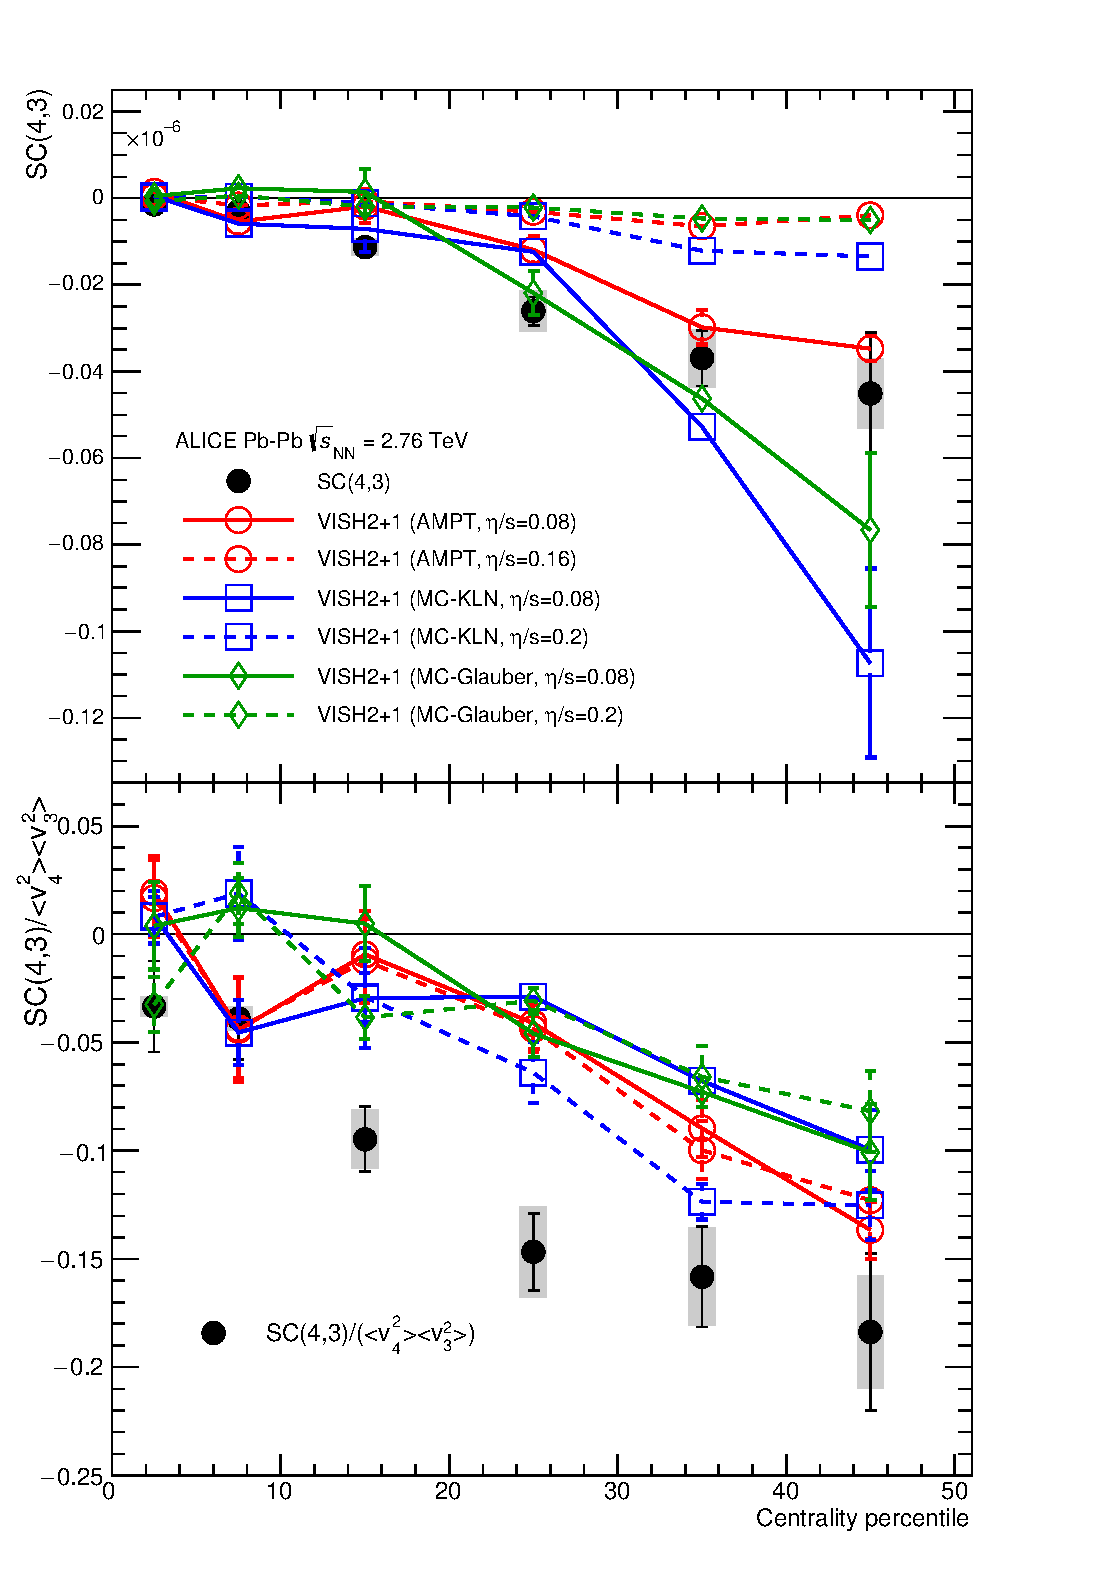
\includegraphics{figures/figs_results/fig3_QConly_ModelComparison_SC43_vish.eps}}
        \caption{Result of  $SC(5,2)$, $SC(5,3)$ and $SC(4,3)$ with ALICE data and comparison to various VISH2+1 calculation with different settings. The configurations are same as Fig.\ref{vish21}}
        \label{vishcomhigh}
        \end{center}   
     \end{figure}

  The event-by-event calculation from VISH by using a hybrid approach based on (2+1)-dimensional viscous hydrodynamics(VISH2+1) were tested and shown in Fig.\ref{vishcomhigh}. All the models with the large share viscosity regardless of the initial conditions ($\eta/s$=0.2 for MC-KLN and MC-Glauber initial conditions, and $\eta/s = 0.16$ for AMPT) failed to capture the centrality dependence of $SC(5,2), SC(5,2)$, and $SC(5,3)$ more clearly than lower order harmonic correlations ($SC(3,2), SC(4,2)$).
And among the models with small shear viscosity ($\eta/s$=0.08), the one from the AMPT initial condition describes the data much better than the other initial conditions. 
A quite clear separation between different initial conditions is observed for these higher order harmonics correlations compared to the lower order harmonic correlations.
$NSC(5,2)$ and $SC(5,3)$ are quite sensitive to both the initial conditions and the $\eta/s$ parametrizations.
As similarly as the above mentioned hydrodynamic calculations~\cite{Niemi:2015qia}, the sign of the $NSC(4,3)$ in these models is opposite to the data in 0-10\% central collisions. NSC(4,3) shows sensitivity to both initial conditions and $\eta/s$ parameterizations while $NSC(3,2)$ didn't show sensitivity to neither initial conditions nor $\eta/s$ parameterizations.
SC(4,3) data is clearly flavoured by smaller $\eta/s$ but NSC(4,3) cannot be described by these models quantitively.






\section{$p_T$ dependence of $SC(m,n)$ and normalized $SC(m,n)$}

To analyze $p_T$ dependence of $SC(m,n)$ and normalized $SC(m,n)$ result, we set various cut conditions for $p_T$ of measuring particles, instead of using all charged hadrons with $0.2 < p_T < 5.0$ GeV/$c$ in $|\eta|<0.8$ region. The simplest approach to analyze $p_T$ dependence is to apply different $p_T$ bin windows when measuring $SC(m,n)$. But the number of particles in each $p_T$ bin groups decreases rapidly as function of $p_T$ and the number of combination for cumulants pair will decrease even more rapidly ($ \sim\frac{1}{n^4}$) and this method causes large statistical fluctuations. Because the original $SC(m,n)$ has only the order of few $10^{-6}$ strength signal, it is not simple to get clear $p_T$ dependence from different $p_T$ window bins from a large statistical fluctuations. To prevent the statistical fluctuation issue, we apply minimum $p_T$ cuts, instead of $p_T$ bin-by-bin windows. In this analysis, we tested $SC(m,n)$s (and also $NSC(m,n)$s) with different $p_T$ conditions from $0.2 \sim 5.0$GeV/$c$ to $1.5 \sim 5.0$GeV/$c$. 
%%done here

The result of $p_T$ dependence with $SC(3,2)$ and $SC(4,2)$ is shown in Fig.\ref{fig:ptdep}. As seen in figure, the strength of $SC(m,n)$ correlation becoming larger as function of minimum $p_T$. This indicates that the relationship between event-by-event fluctuation of two different flow harmonics $v_m$ and $v_n$ is stronger in high $p_T$ region. This $p_T$ dependence correlation is relatively small in central collision centralities and large in non-central collisions. However, this correlation between flow harmonics and $p_T$ is not clearly shown in $NSC(m,n)$s. The  $NSC(m,n)$ results are aligned all together and consistent within errors. The ratio to default cut ($0.2 < p_T < 5.0$GeV/$c$) is nearly 1 for all centrality. This suggests that the $p_T$ dependence of $SC(m,n)$ are not solely comes from the correlation between flow harmonics but comes from the strength dependence of $p_T$ of single $v_n$ values. Minimum $p_T$ cuts are extended to 1.5 GeV/$c$ and the results are shown in Fig.\ref{fig:ptdephigh}. Even in higher minimum $p_T$ cuts, there is no clear $p_T$ dependence in normalized $SC(3,2)$ or $SC(4,2)$. For detail study of $p_T$ dependence of  $NSC(m,n)$, the $NSC(m,n)$ as function of minimum $p_T$ cuts are prepared in Fig.\ref{fig:SC_xpt}. Unlike AMPT prediction, the results from the data does not have clear $p_T$ dependence up to 40\% collision centralities. In 40-50\% collision centrality region, there is a slightly decreased slope in $NSC(3,2)$ but it is not enough to say that there is $p_T$ dependence for $NSC(3,2)$. For AMPT simulations, AMPT with string melting configuration failed to capture data result. These AMPT simulation predict that normalized $SC(m,n)$ increase as a function of minimum $p_T$ and turns over to positive values around minimum $p_T \sim 1.0$GeV/$c$. But in LHC10h data, the results remains in negative values for all minimum $p_T$ bins, and centrality bins. Also for $NSC(4,2)$ cases, only AMPT default which has the configuration without string melting, has similar values with data. The others (AMTP with string melting) predict increase of $NSC(4,2)$ from around $\sim 1$GeV/$c$ minimum $p_T$ cuts, and failed to reproduce the data.

	\begin{figure}[p]
		\begin{center}
        	\resizebox{0.6\columnwidth}{!}{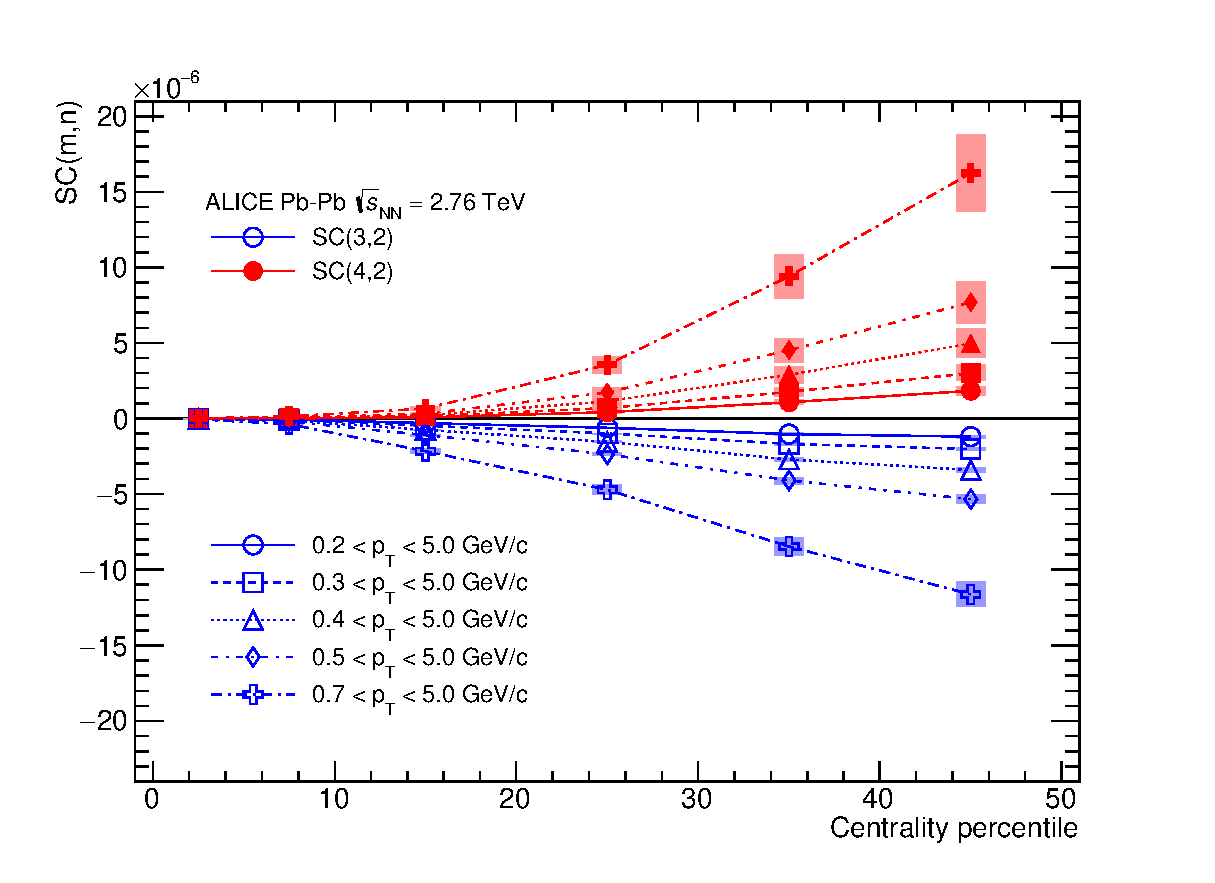
\includegraphics{figures/figs_results/fig4_QConly_SC_ptdep}}
        	\resizebox{0.6\columnwidth}{!}{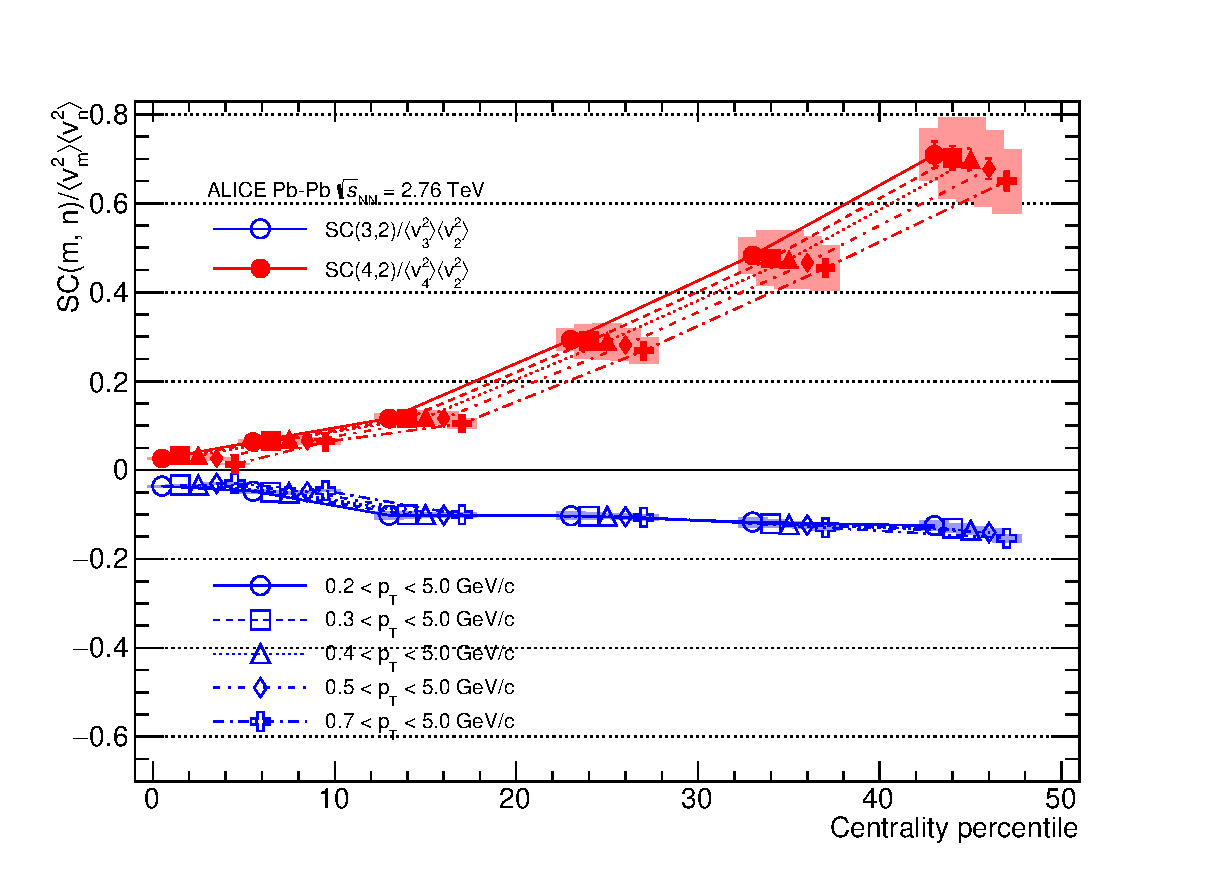
\includegraphics{figures/figs_results/fig4_QConly_nSC_ptdep}}
        	\resizebox{0.6\columnwidth}{!}{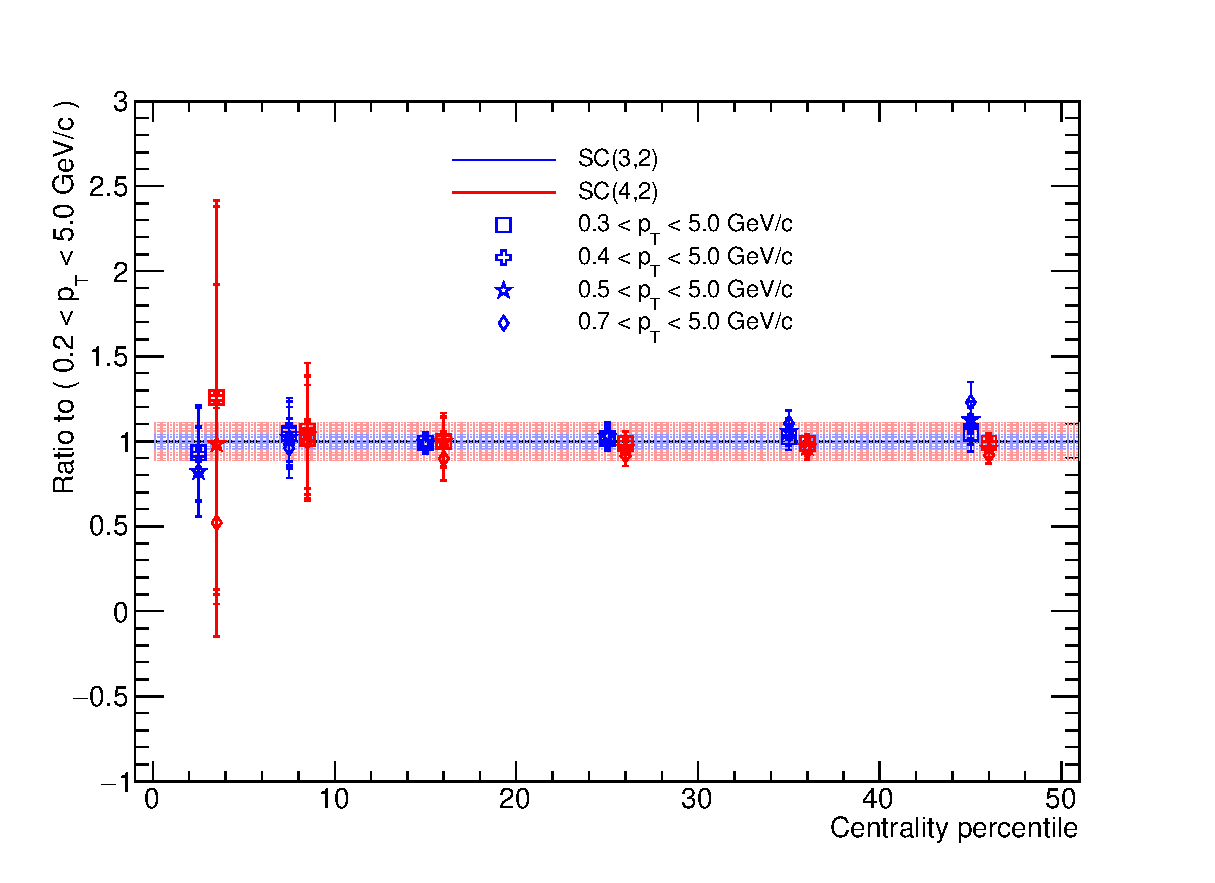
\includegraphics{figures/figs_results/fig4_QConly_nSC_ptdep_ratio}}
        \caption{The results of $SC(3,2)$ and $SC(4,2)$ with various minimum $p_T$ cut conditions(Top) and results of  $NSC(3,2)$ and $NSC(4,2)$(Middle). The ratio of $NSC(m,n)$ results with various minimum $p_T$ cut conditions to default($0.2 < p_T < 5.0$GeV/$c$ are shown in bottom figure.}
        \label{fig:ptdep}
        \end{center}   
     \end{figure}


	\begin{figure}[p]
		\begin{center}
        	\resizebox{0.6\columnwidth}{!}{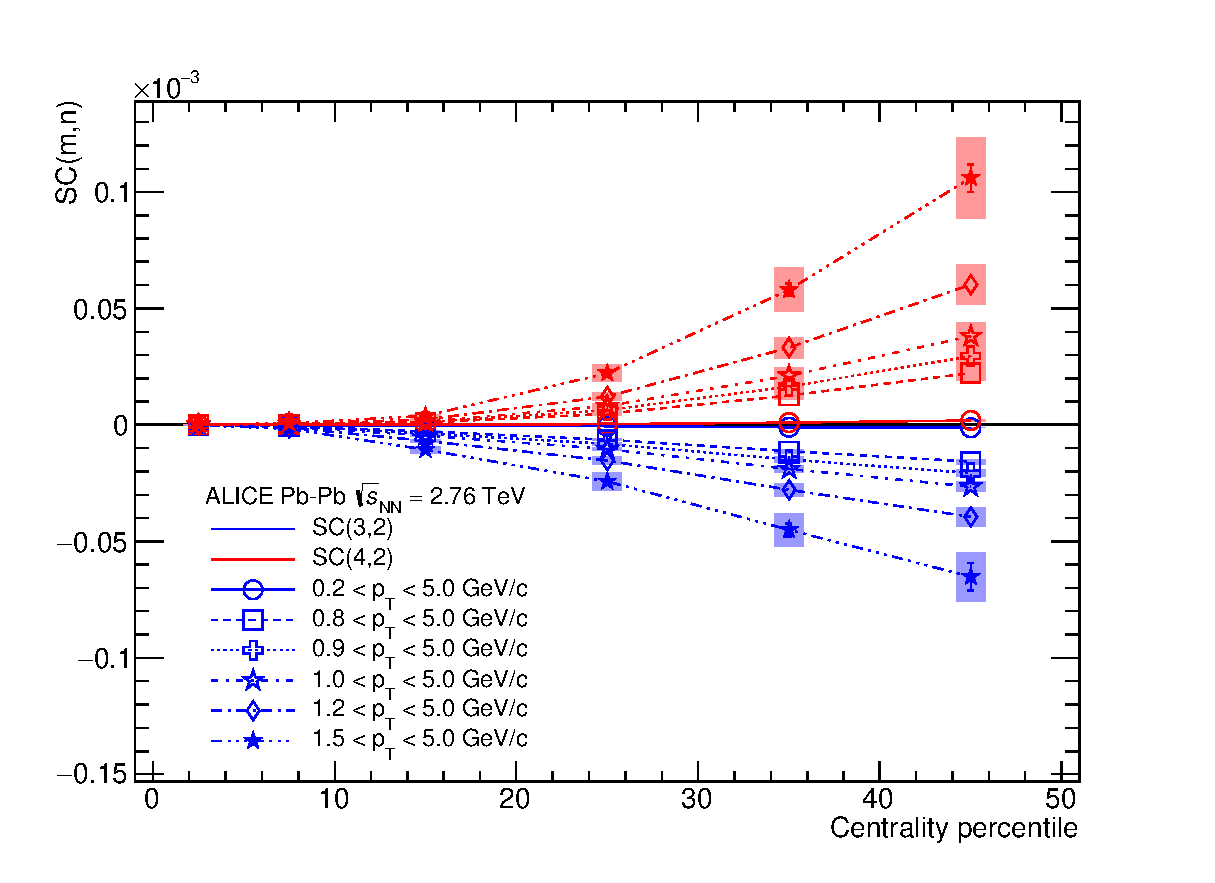
\includegraphics{figures/figs_results/fig4b_QConly_SC_ptdep}}
        	\resizebox{0.6\columnwidth}{!}{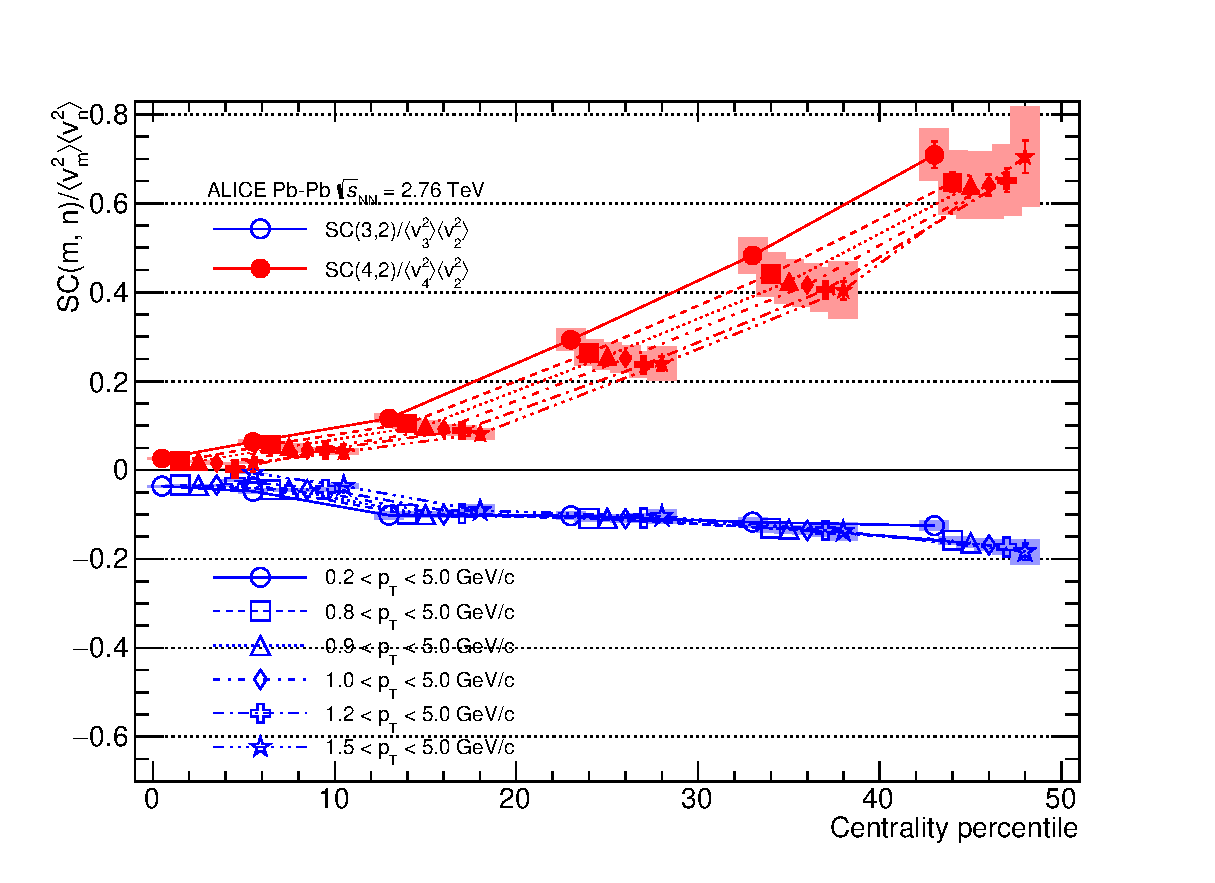
\includegraphics{figures/figs_results/fig4b_QConly_nSC_ptdep}}
        	\resizebox{0.6\columnwidth}{!}{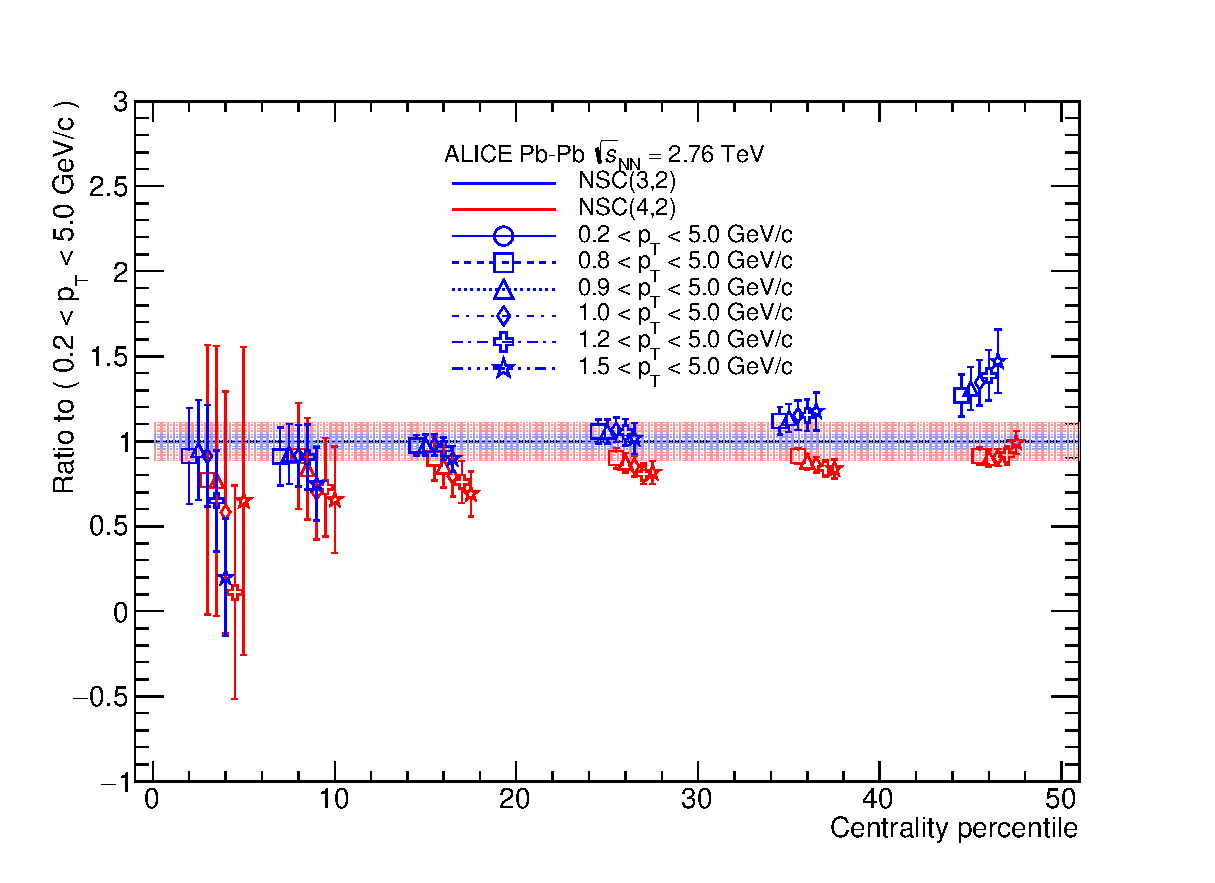
\includegraphics{figures/figs_results/fig4b_QConly_nSC_ptdep_ratio}}
        \caption{The results of $SC(3,2)$ and $SC(4,2)$ with various minimum $p_T$ cut conditions(Top) and results of  $NSC(3,2)$ and $NSC(4,2)$(Middle). The ratio of $NSC(m,n)$ results with various minimum $p_T$ cut conditions to default($0.2 < p_T < 5.0$GeV/$c$ are shown in bottom figure.}
        \label{fig:ptdephigh}
        \end{center}   
     \end{figure}


	\begin{figure}[p]
		\begin{center}
        	\resizebox{0.95\columnwidth}{!}{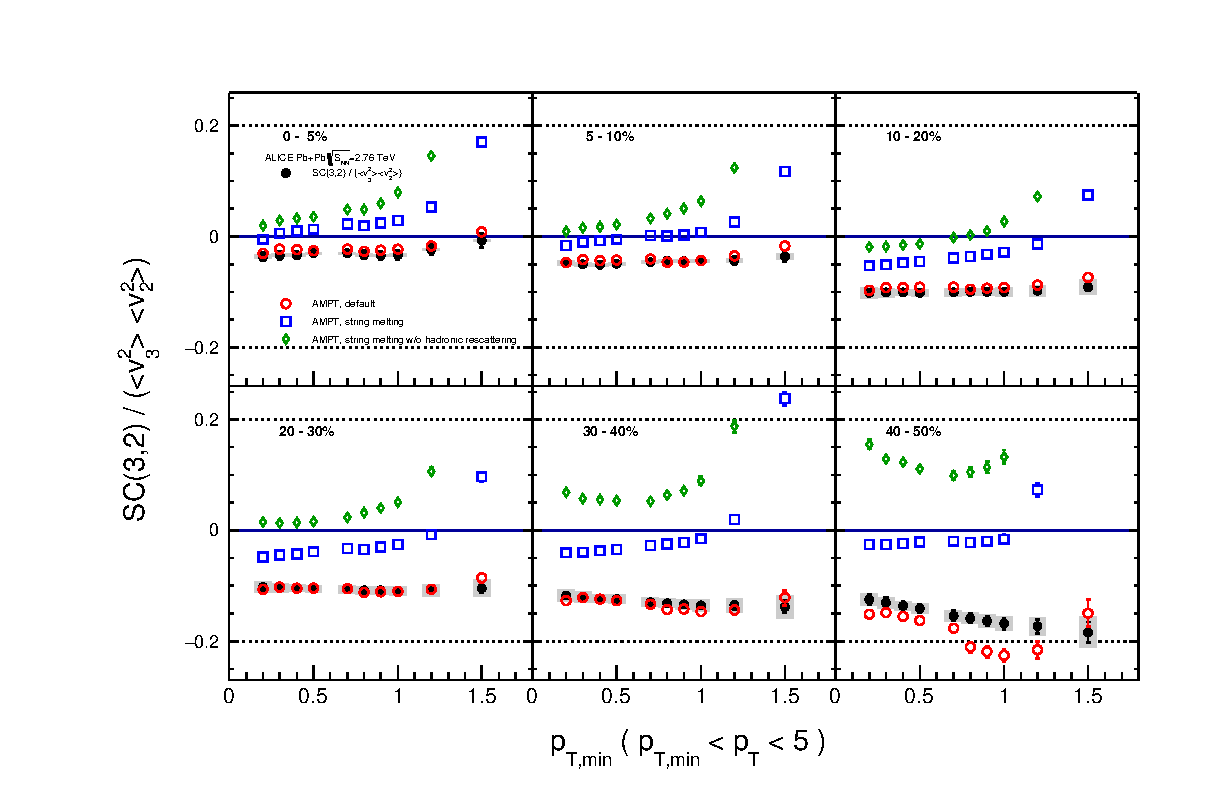
\includegraphics{figures/figs_results/fig5_QConly_xminpt_nSC32}}
        	\resizebox{0.95\columnwidth}{!}{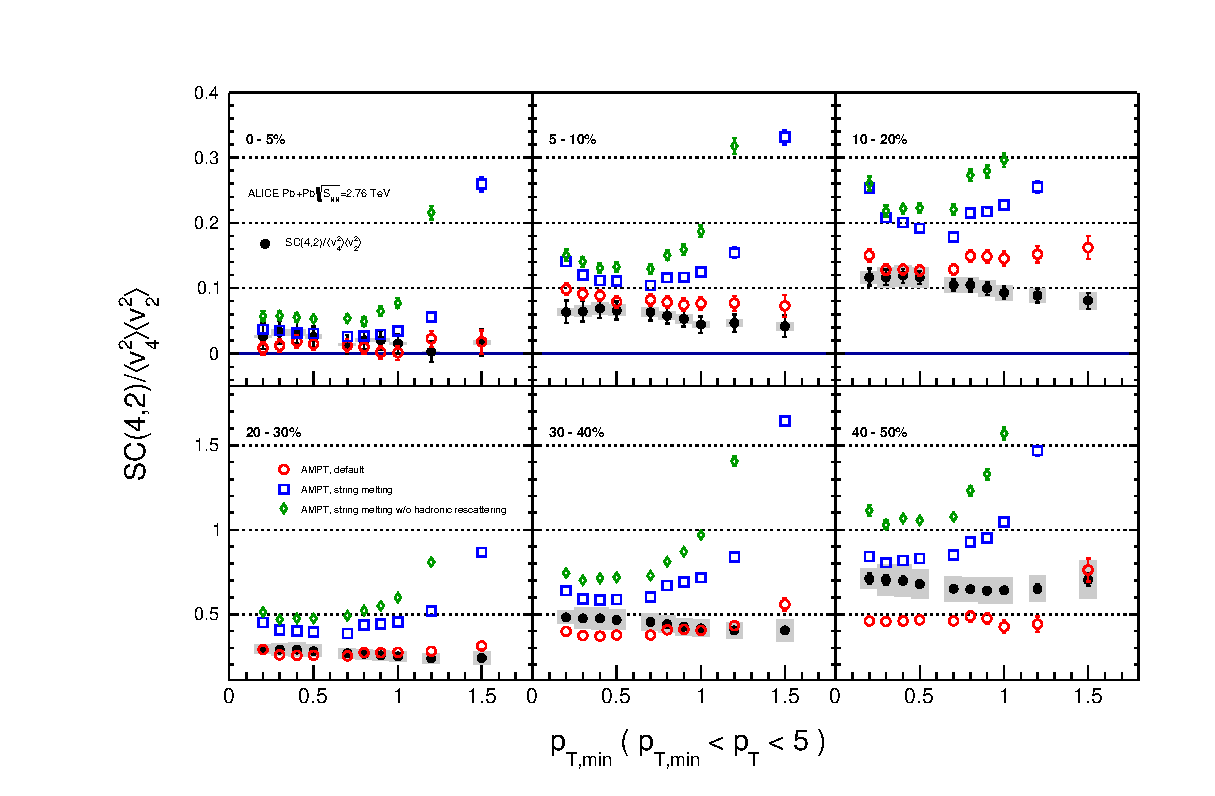
\includegraphics{figures/figs_results/fig5_QConly_xminpt_nSC42}}
           \caption{$NSC(3,2)$(Top) and $NSC(4,2)$(Bottom) as a function of minimum $p_T$ cuts with ALICE Pb+Pb $\sqrt{S_{NN}}=2.76$TeV. The AMPT simulation results are drawn together as colored band for comparison. The corresponding AMPT configurations are shown in legend.}
        \label{fig:SC_xpt}
        \end{center}   
     \end{figure}
\clearpage

%done here


\section{Method comparison}


The Eq.\ref{eq:SC} is based on the multi-particle q-Cumulants method(i.e. QC method), but it can be also obtained by calculating moments \cite{Bhalerao:2015jg} as discussed in the previous section\ref{sec:analysis}.


	\begin{figure}[bp]
		\begin{center}
        	\resizebox{0.47\columnwidth}{!}{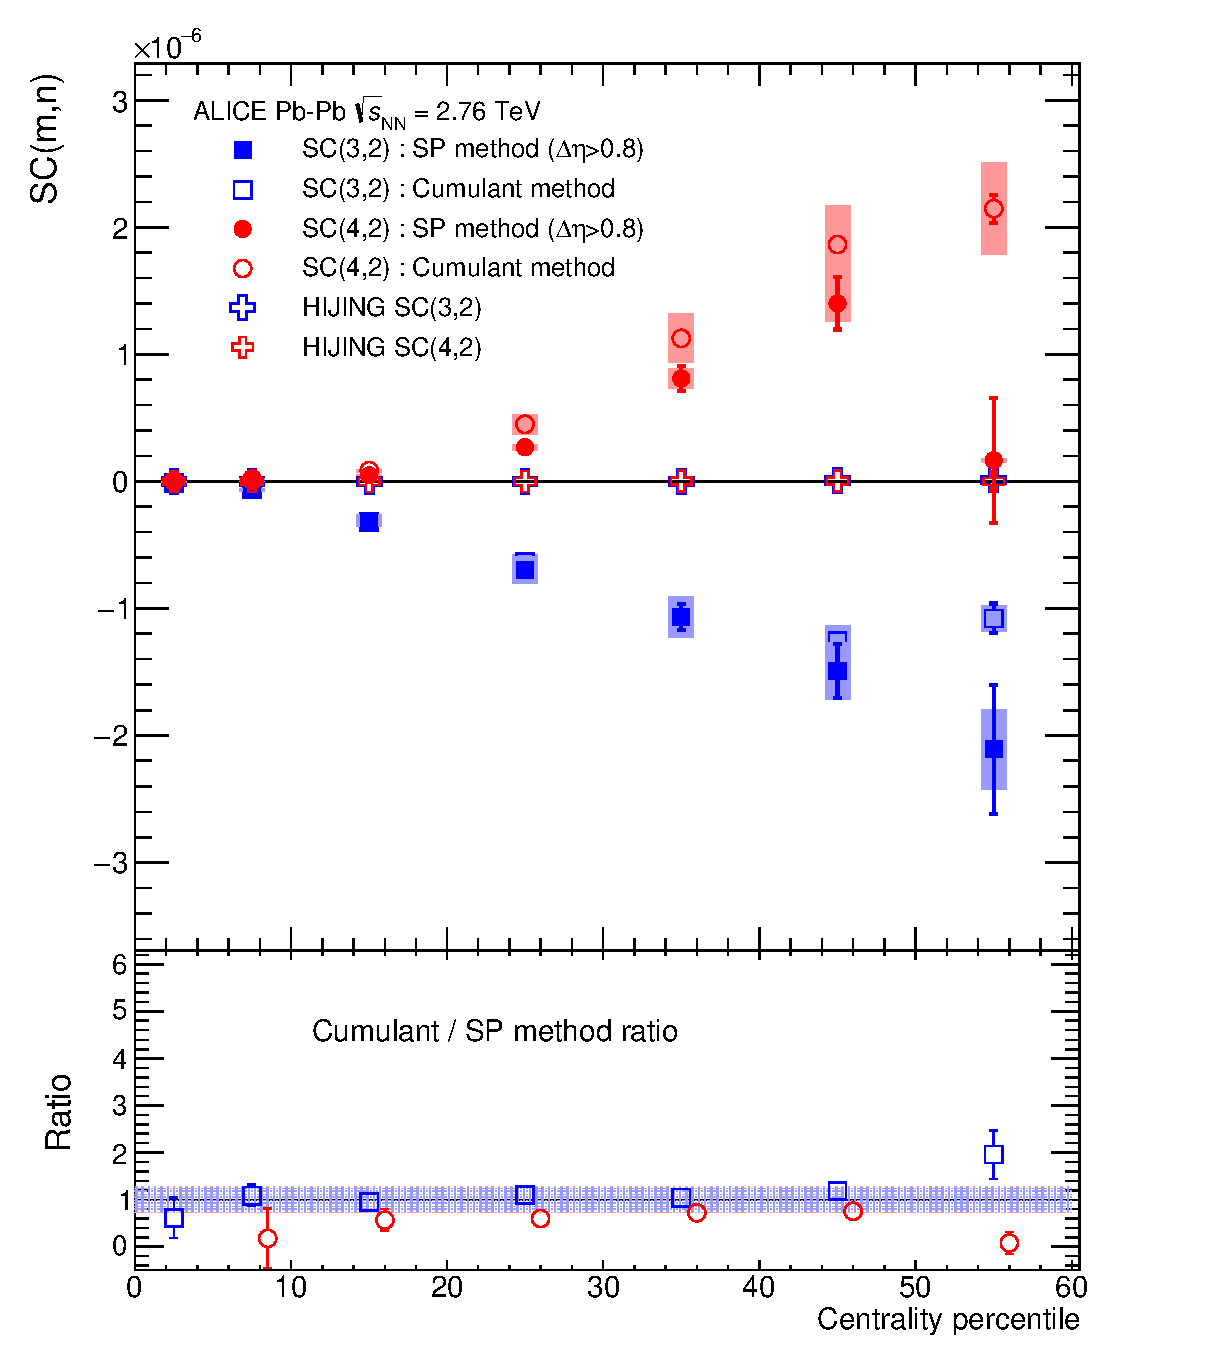
\includegraphics{figures/figs_compare_with_SP/fig1a}}
        	\resizebox{0.47\columnwidth}{!}{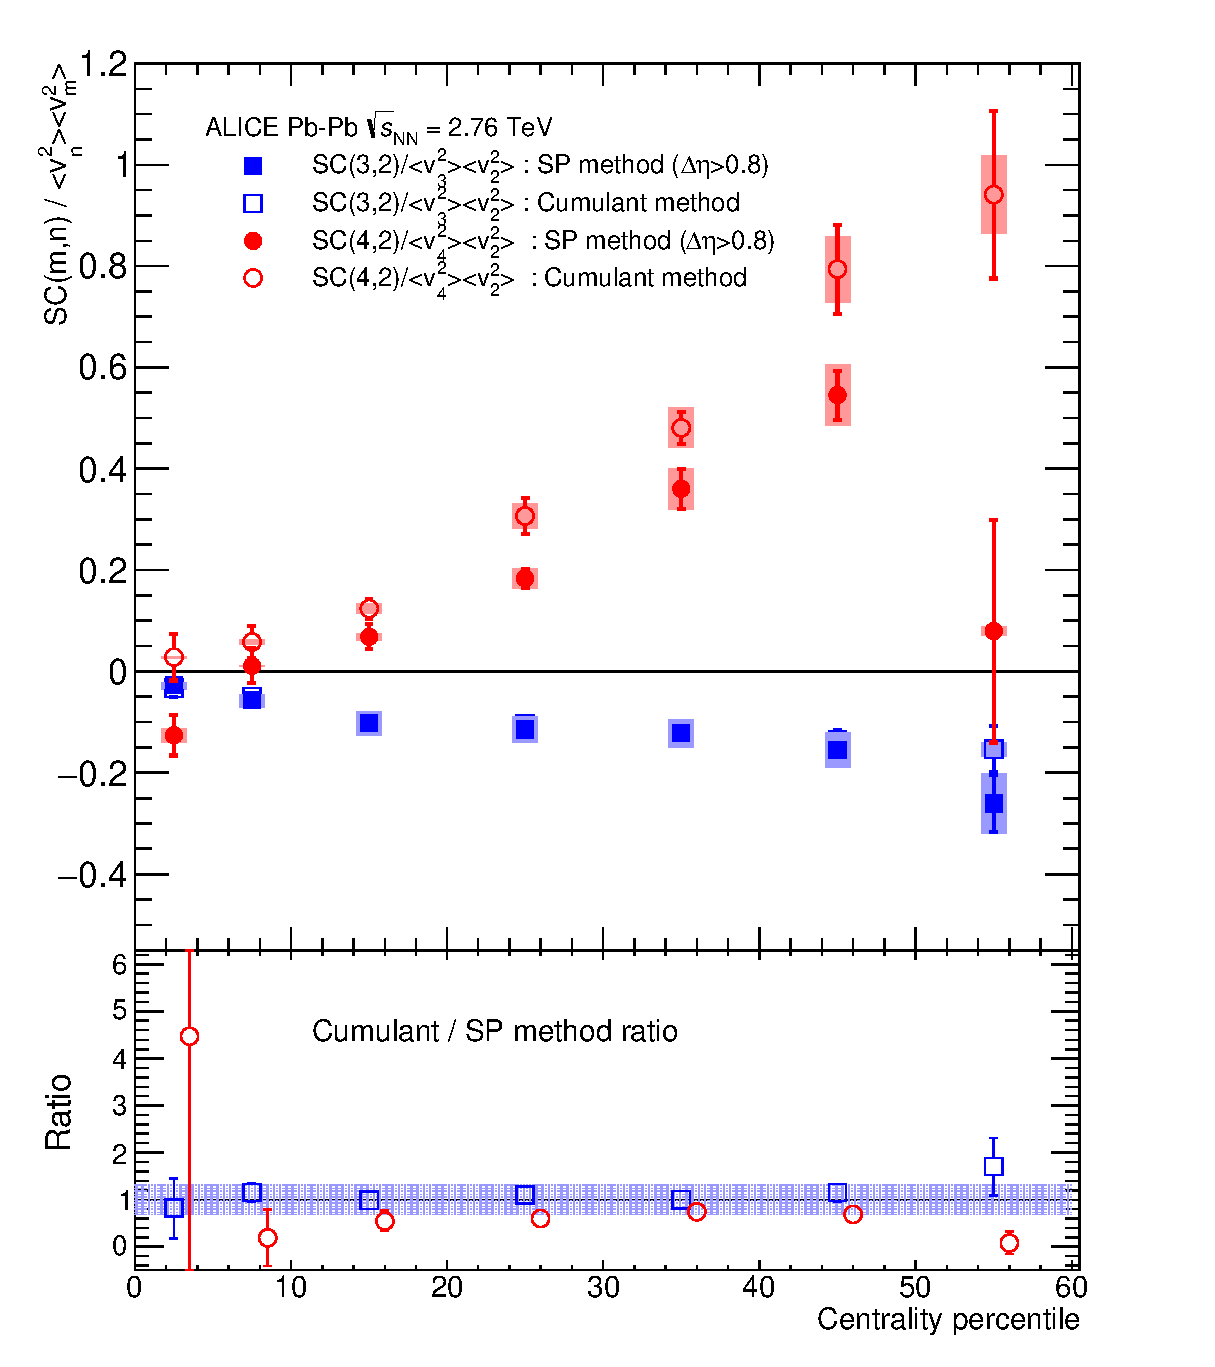
\includegraphics{figures/figs_compare_with_SP/fig1b.eps}}
        \caption{Comparison of $SC(m,n)$(Top) and normalized $SC(m,n)$(Bottom) results for $SC(3,2)$(blue) and $SC(4,2)$(red) with the SP and QC method up to 60\% centralities. The different ratios are shown in lower pads, and systematic uncertainty is drawn as a band around 1}
        \label{SC_compare}
        \end{center}   
     \end{figure}


As seen in Fig.\ref{SC_compare} in both methods, the flow harmonics with 2nd and 4th are correlated. On the other hand, 2nd and 3rd harmonics are anti-correlated. The strength of correlation is small in the central collision region and becomes stronger in non-central collision in both q-Cumulant method(QC) and Scalar Product method(SP). Also  $NSC(m,n)$ which is divided by products $\langle v_m^2 \rangle \langle  v_n^2\rangle$, in order to obtain the normalized observables are shown and suggests the same trend but a large deviation especially for $SC(4,2)$. HIJING simulations results from SP methods are shown together for comparison. 

The advantage of using the SP method is that calculations are much simpler and faster in estimating the correlation between flow harmonics. Instead of calculating particle pair of 4- or 2- cumulants, the SP method needs only one calculation between measured n$^{th}$ order flow $Q$-vector. The other advantage of the SP method is that it can be applied for not only $SC(m,n)$ which observables for flow ``magnitudes" correlation, but also for the flow "direction" correlations like event-plane correlation. \cite{Aad:2014fla} or non-linear response of flow harmonics \cite{Yan:2015dh}. 

However, the disadvantage of SP methods is (likely) under estimation of $SC(m,n)$ in low multiplicity regions. This effects were discussed with ToyMC simulation in Appendix A. Because of this issue of difference between two different methods and inaccuracy(under estimation) of SP method in low multiplicity regions, we used all the result from QC method as the default in this analysis.


\subsubsection{Method comparison of higher order harmonics}


Also $SC(m,n)$ and $NSC(m,n)$ results with higher order flow harmonics (up to 5th order) were measured by the SP method, and the results are shown in Fig.\ref{SC_higherorder_comparison}. For the higher order, because of statistical fluctuation for peripheral collisions, results were only taken from the 0\% to 40\% collision centrality regions. As a result, the two methods shows the consistent values within errors.


	\begin{figure}[h]
		\begin{center}
        	\resizebox{0.65\columnwidth}{!}{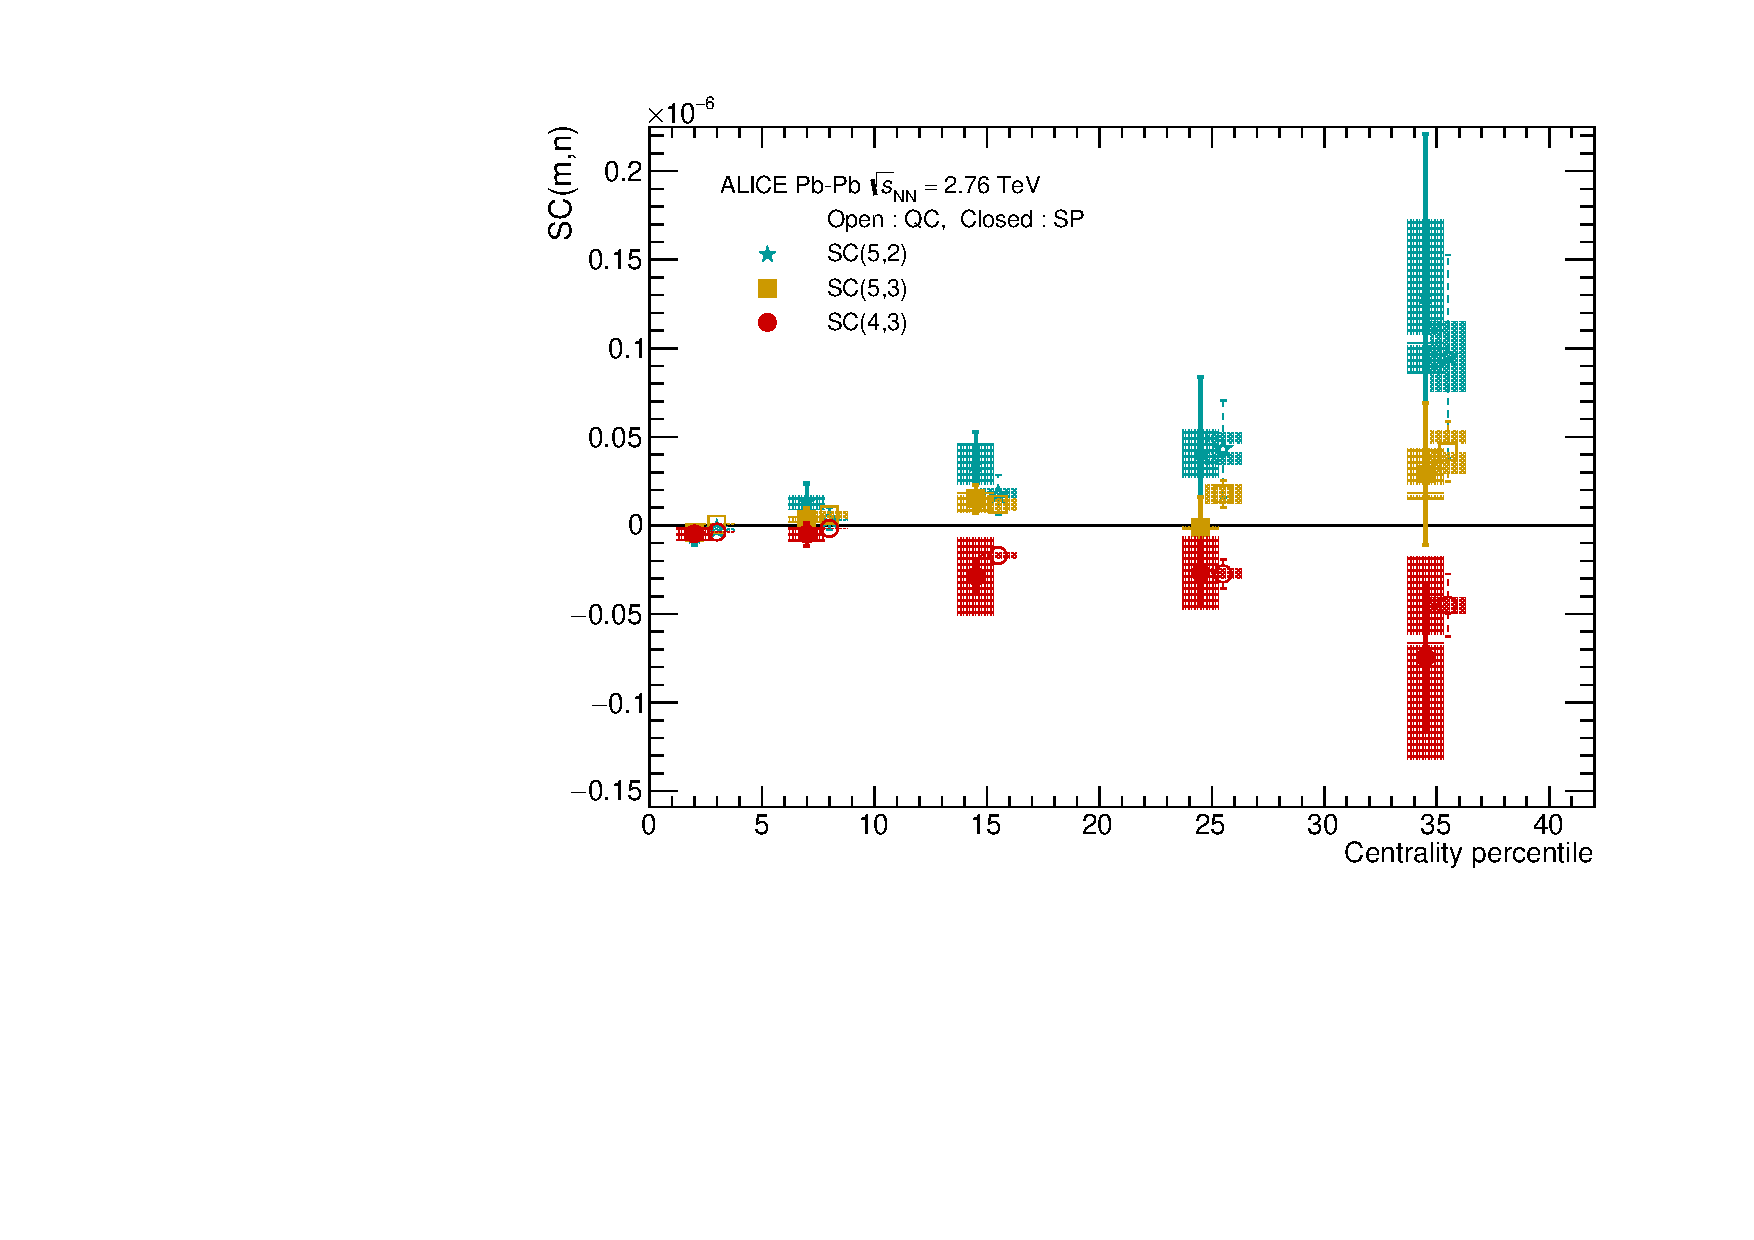
\includegraphics{figures/figs_compare_with_SP/fig2b_1}}
        	\resizebox{0.65\columnwidth}{!}{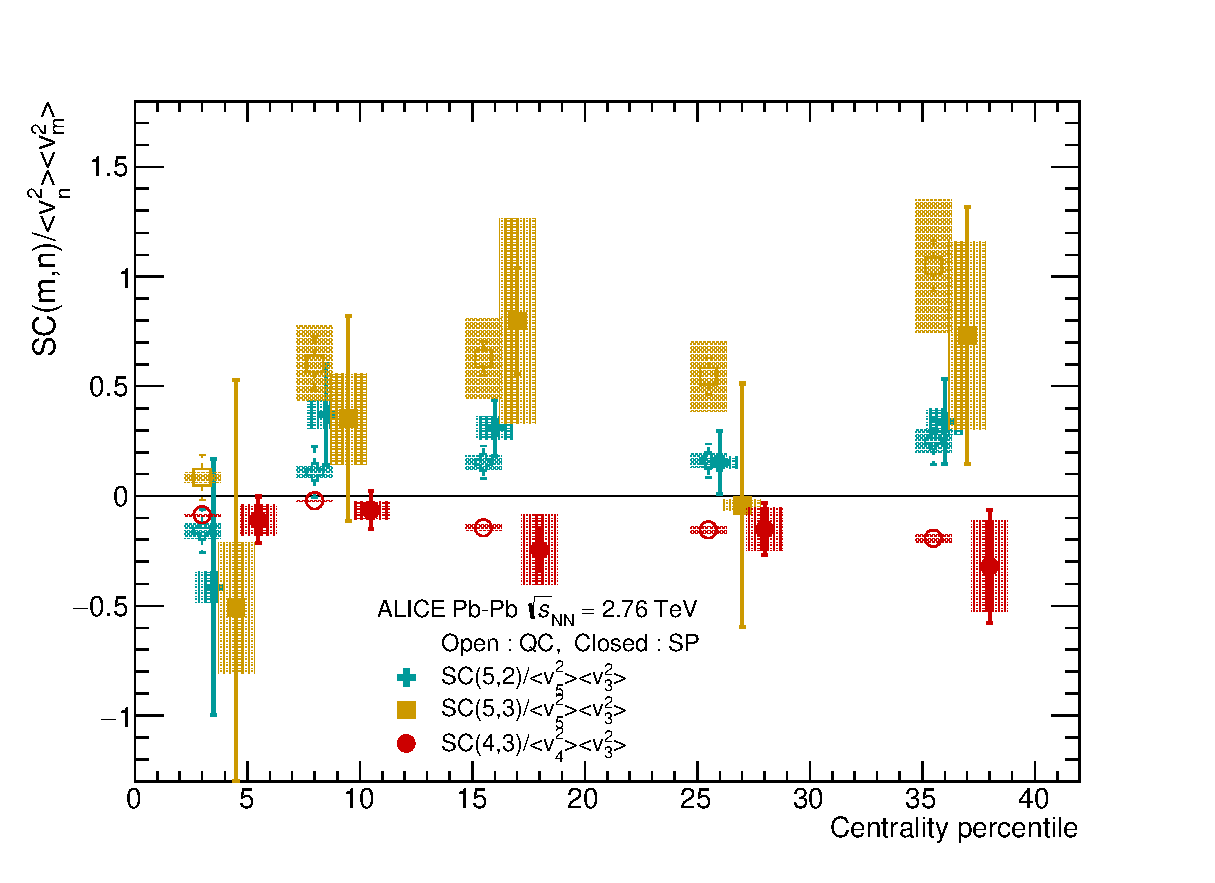
\includegraphics{figures/figs_compare_with_SP/fig2b_2}}
        \caption{Result of higher order $SC(m,n)$ and $NSC(m,n)$ with two different method QC and SP. Along x-axis offset was applied for better visibility. For the QC method $|\eta| < 0.8$ cut was applied, while SP method takes $0.4 < |\eta| <0.8$.}
        \label{SC_higherorder_comparison}
        \end{center}   
     \end{figure}
     
     
\subsubsection{$p_T$ dependence of $SC(m,n)$ with SP method}


  The $p_T$ dependence of $SC(m,n)$ and $NSC(m,n)$ were checked with the SP method. The results of $SC(m,n)$ and $NSC(m,n)$ with different minimum $p_T$ cuts are shown in Fig.\ref{fig:SC_pt_withSP_lower}( up to 0.7 GeV/$c$ minimum $p_T$ cuts) and Fig.\ref{fig:SC_pt_withSP_higher}( up to 1.5 GeV/$c$ ) minimum $p_T$ cuts. As seen in Fig.\ref{fig:SC_pt_withSP_lower}, there is certain $p_T$ dependence for $SC(m,n)$, but not clear $p_T$ dependence for  $NSC(m,n)$ as like QC method. However, in even higher $p_T$ region(Fig.\ref{fig:SC_pt_withSP_higher}), unlike the results with QC methods, we could see weak $p_T$ dependence in  $NSC(m,n)$. In the $SC(m,n)$ results, as the minimum $p_T$ cuts goes higher, the strength of the correlation becomes stronger in both $SC(3,2)$ and $SC(4,2)$. However, in $NSC(m,n)$ with the SP method, when the minimum $p_T$ cuts increase, the strength of correlation for $NSC(3,2)$ is (negatively) stronger, but the strength of correlation of $NSC(4,2)$ becomes weaker. As a result, in higher $p_T$ range, the $NSC(m,n)$ values always getting smaller.


	\begin{figure}[htbp]
            \begin{center}
                       \resizebox{0.84\textwidth}{!}{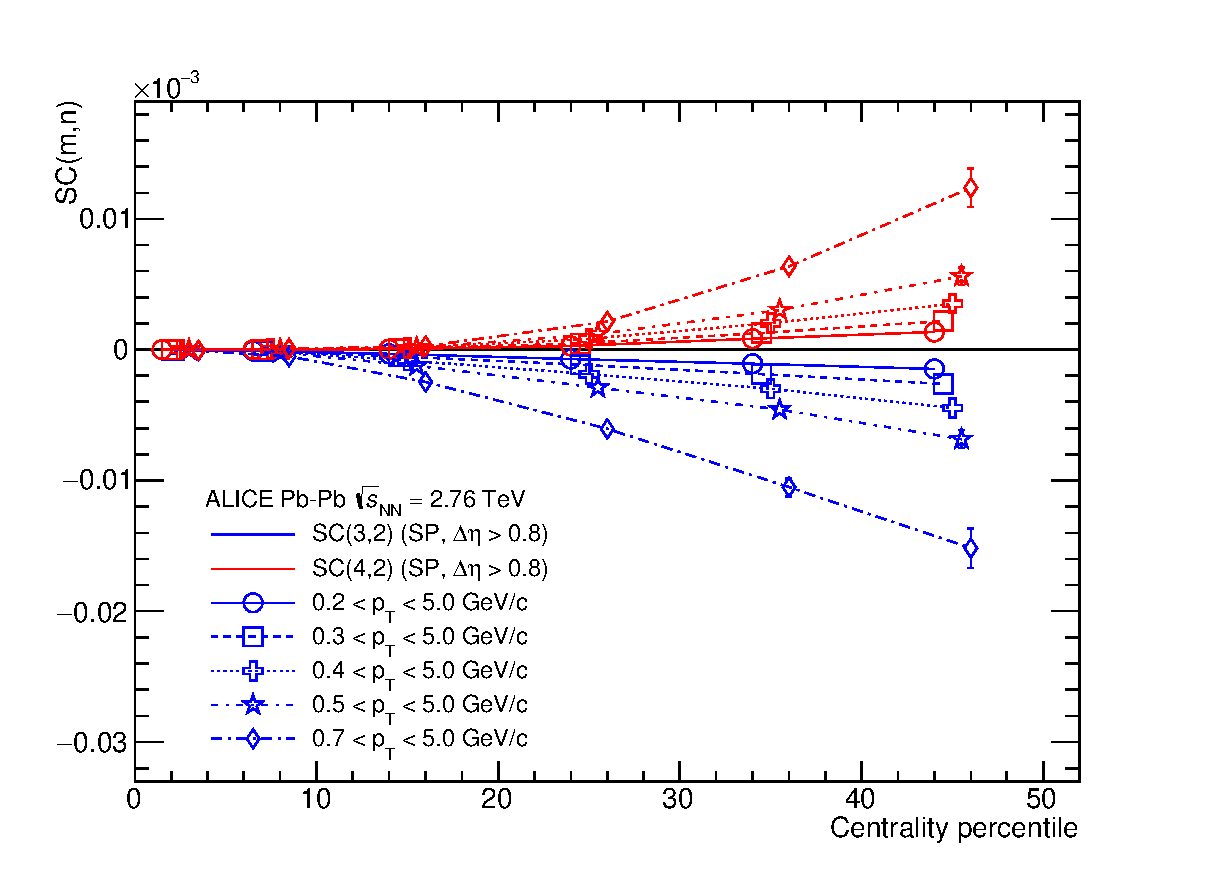
\includegraphics{figures/figs_compare_with_SP/fig3a.eps}}
                       \resizebox{0.84\textwidth}{!}{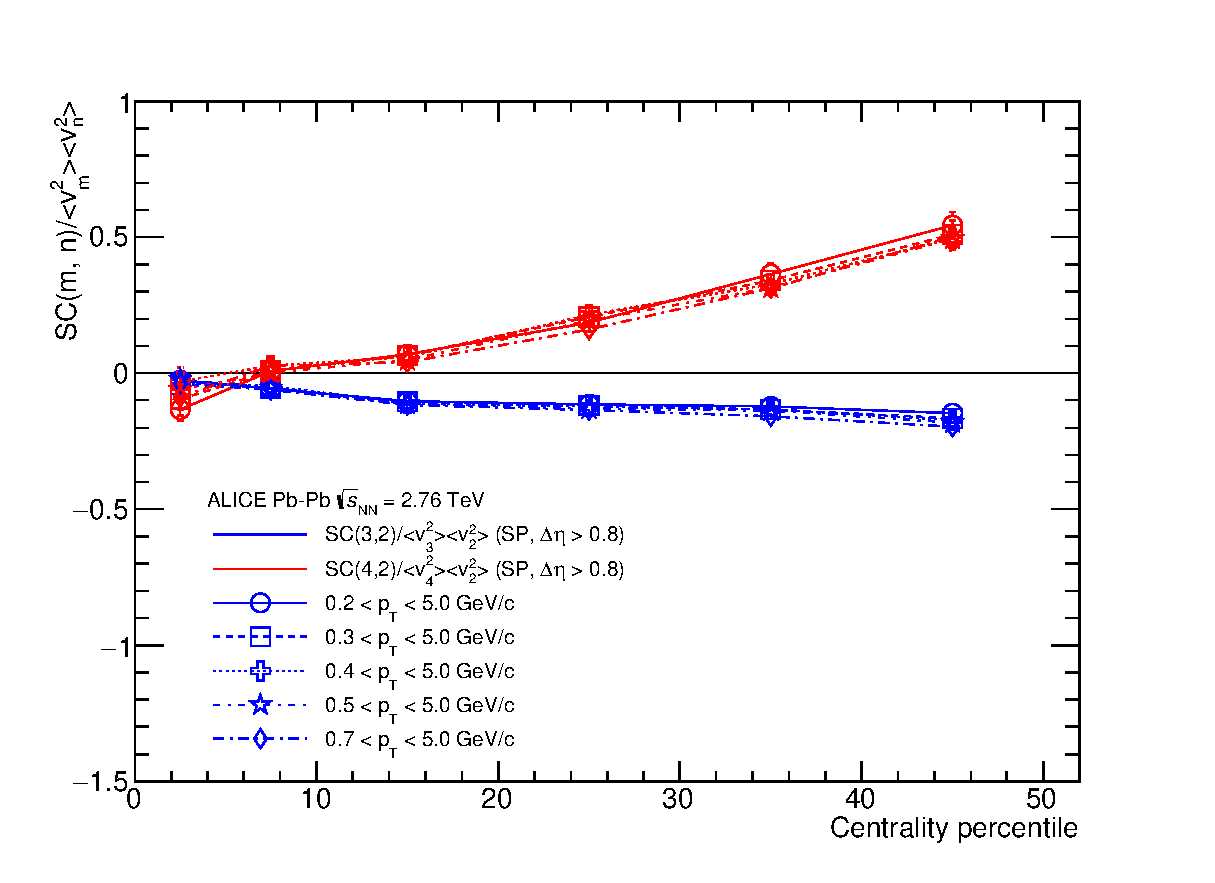
\includegraphics{figures/figs_compare_with_SP/fig3b.eps}}
              \end{center}
              \caption{$SC(m,n)$ and $NSC(m,n)$ with SP method with default cuts ( 0.2 < $p_T$ < 5.0 GeV/$c$ ) and various minimum $p_T$ cuts up to 0.7 GeV/$c$ }
              \label{fig:SC_pt_withSP_lower}
       \end{figure}


	\begin{figure}[htbp]
            \begin{center}
                       \resizebox{0.84\textwidth}{!}{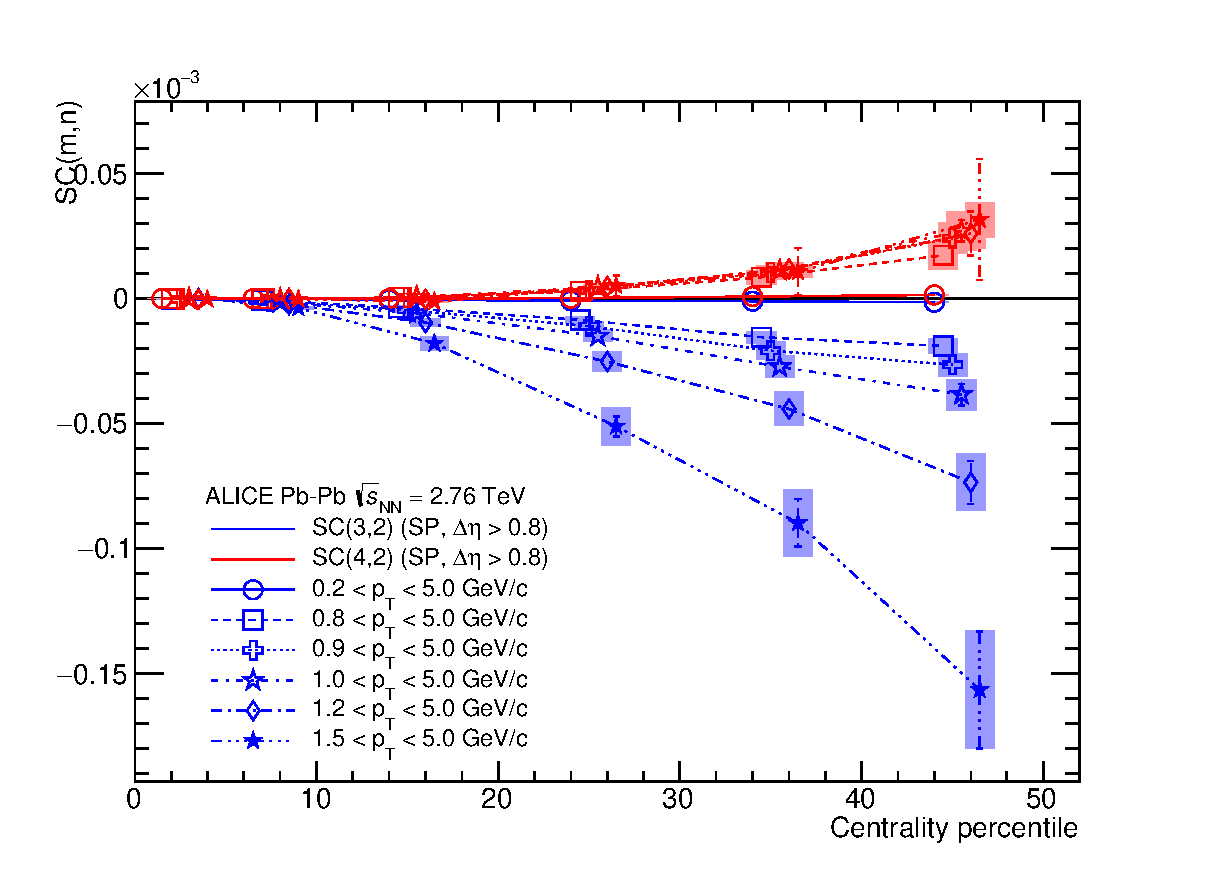
\includegraphics{figures/figs_compare_with_SP/fig3a_higherpt.eps}}
                       \resizebox{0.84\textwidth}{!}{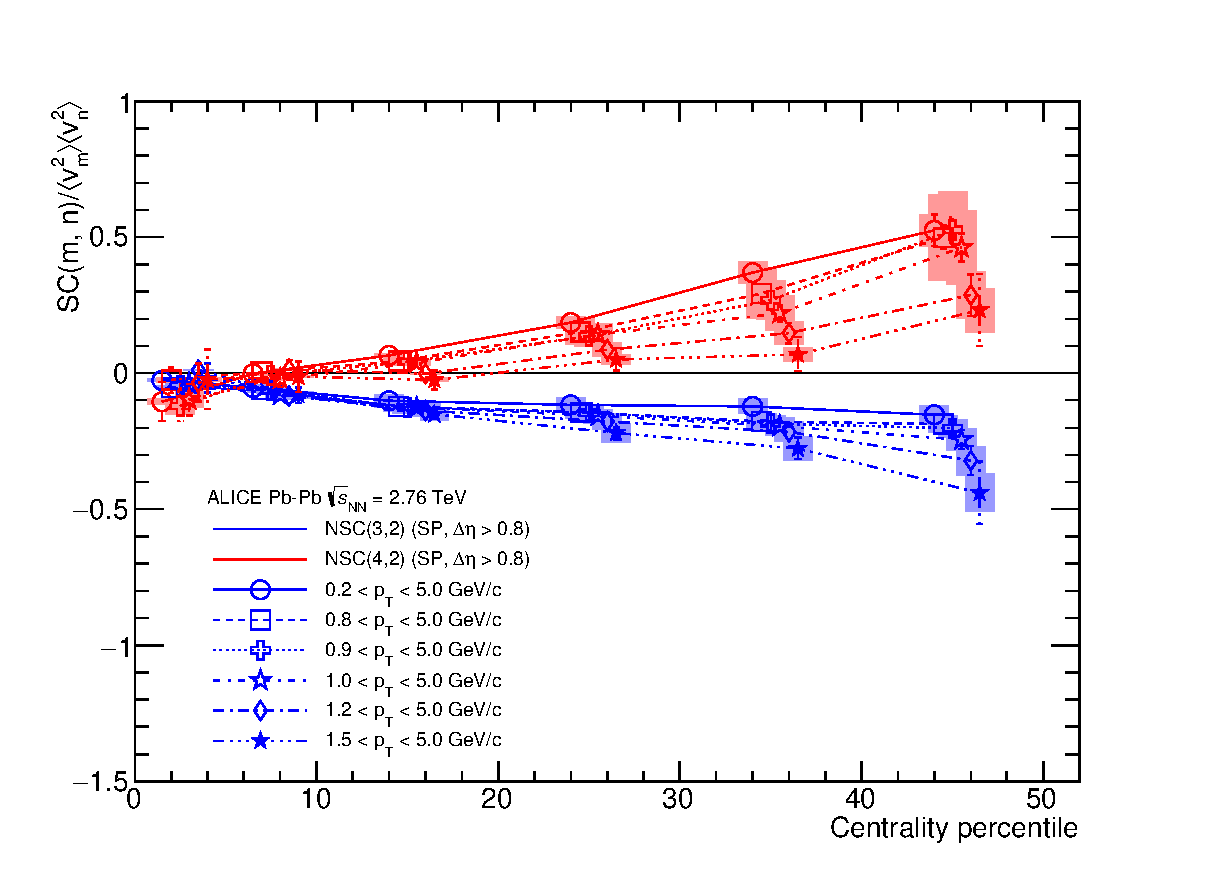
\includegraphics{figures/figs_compare_with_SP/fig3b_higherpt.eps}}
              \end{center}
              \caption{$SC(m,n)$ and $NSC(m,n)$ with SP method with default cuts ( 0.2 < $p_T$ < 5.0 GeV/$c$ ) and various minimum $p_T$ cuts up to 1.5 GeV/$c$ )}
              \label{fig:SC_pt_withSP_higher}
       \end{figure}



	\begin{figure}[htbp]
            \begin{center}
                                     \resizebox{0.84\textwidth}{!}{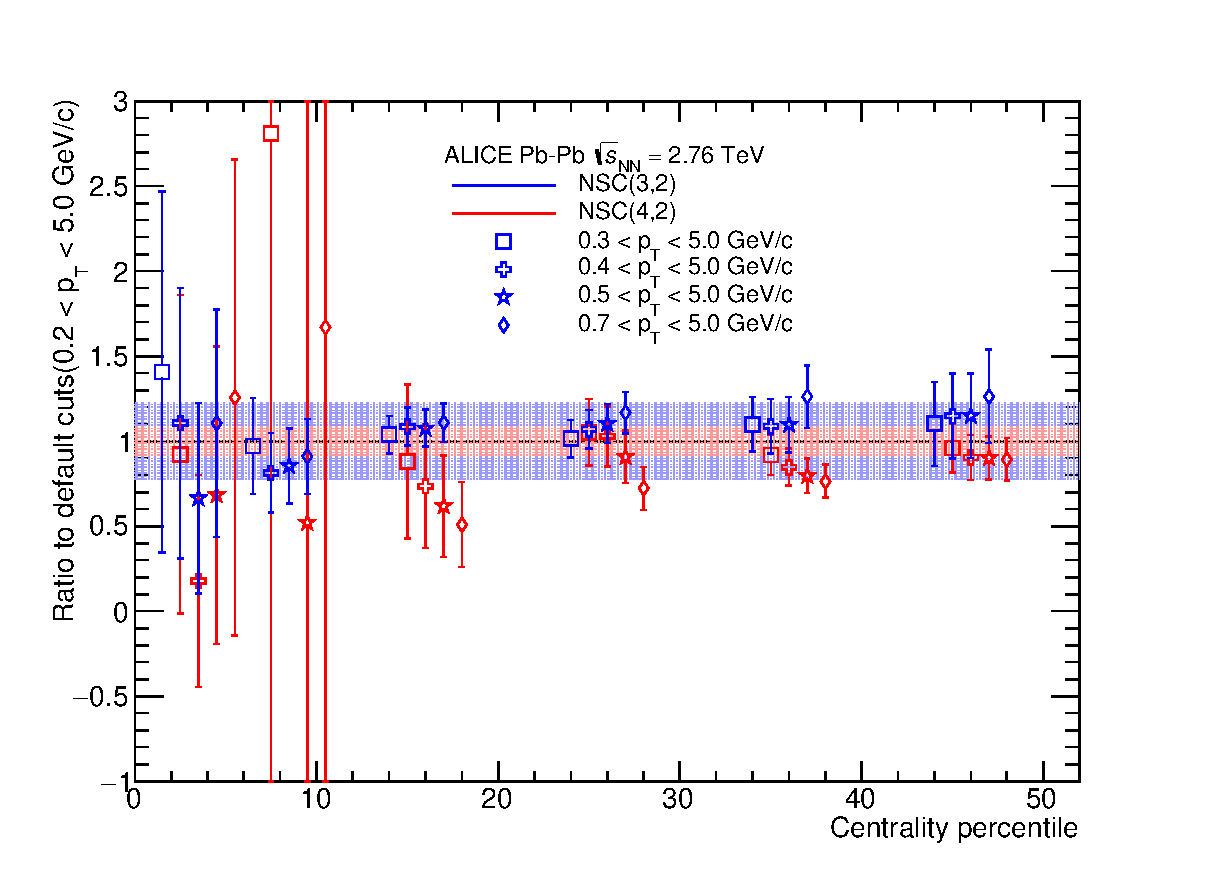
\includegraphics{figures/figs_compare_with_SP/fig3c.eps}}
                                     \resizebox{0.84\textwidth}{!}{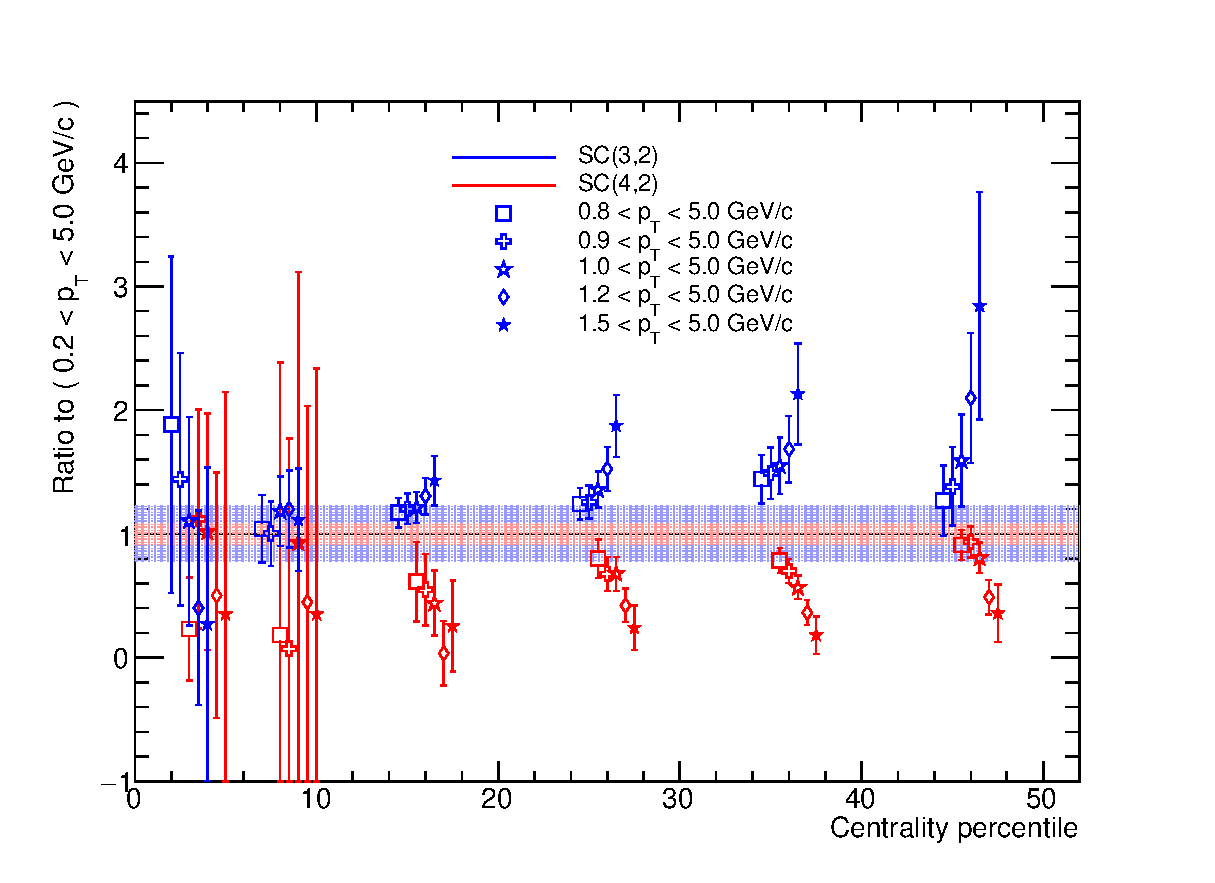
\includegraphics{figures/figs_compare_with_SP/fig3c_higherpt.eps}}
              \end{center}
              \caption{ The ratio of $NSC(m,n)$ with SP method to the default cuts }
              \label{fig:SC_pt_withSP_ratio}
       \end{figure}

  For the better comparison, the ratio of normalized $SC(m,n)$ with various minimum $p_T$ cuts to default is shown in Fig.\ref{fig:SC_pt_withSP_ratio}. Up to 0.7 GeV/c, the ratio of $NSC(m,n)$ values are consistent with a default cut within errors, but the minimum $p_T$ exceeds 0.8GeV/c, the ratio of $NSC(3,2)$ moving above the 1, and the ratio of $NSC(4,2)$ goes down below the 1. The reason why these trends are only shown in the SP method, and not in the QC is not yet fully explained. However, the disadvantage of the SP method is that we lose almost half of the statistics because of a large $\eta$ gap around $\eta=0$ and also the number of combinations for the track pair is $\frac{1}{3}$ when compared to QC methods. This is one possible option to explain these $p_T$ dependence behavior of SP method, and  tested in ToyMC simulation in Appendix A.

